\chapter{Introduction} \label{chapter:introduction}
\newpage
\mbox{}
\newpage
\section{The History of Our Understanding of Proteins}

The development of humankind into a social species caused the co-development of tasks distribution and specialisation \cite{masclans_sexual_2021, waguespack_organization_2005, fargher_comparison_2009}. Consequently, we evolutionarily understood that every member in society plays a role in its sustenance. People therefore became workers, with skills and responsibilities developed to fulfil the needs of a societal-forged organism: a community. We probably realised rather early that with experience we could develop expertise, and therefore increase the efficiency of a process, which resulted in specialisation. Guilds, chain production, and academic education are testimonies of work specialisation, which have shaped the society we live in today. Our social specialisation interestingly followed processes homologous to those executed by evolution for billions of years.

In its simplest expression, evolution acts based on three elements: a replication mechanism, a source of variation, and environmental selective pressure \cite{lewontin_units_1970}. An organism that wants to survive for generations must first produce such generations by creating \gls{offspring}. Its \gls{offspring} will inherit their genetic material, generally in Deoxiribonucleic Acid (\gls{dna}) form, which contains the information to execute and regulate the production of all its proteins. The process of producing proteins from information encoded in \gls{dna} is explained in the central dogma of molecular biology, which in its core states that \gls{dna} is transcribed into Ribonucleic Acid (\gls{rna}), subsequently translated into proteins (\figref{fig:chapter1:central_dogma}). The information needed to produce proteins and regulatory elements is encoded by \glspl{gene}, which can be regulated to adjust its expression. The entirety of genetic elements in an organism, including \glspl{gene}, regulatory elements, and other regions constitutes the genetic makeup of such organism, known as \gls{genotype}. Replication of genetic material is error-prone and introduces mutations in the \gls{offspring}'s \gls{genotype}, which may result in \glspl{phenotype} (\textit{i.e.} the \gls{genotype}'s expression in a given environment) variations between the two generations. These differences, \textit{per se}, do not universally improve or deteriorate the fitness of an organism, but they can provide an advantage or handicap under certain environmental conditions \cite{luzzatto_sickle_2012, uyoga_sickle_2022}. \Gls{offspring} with favourable traits will have a higher chance of surviving and of producing subsequent \gls{offspring}, a process which iterates over generations, continuously selecting traits that are beneficial and adapted to the environment \cite{noauthor_natural_nodate} (Figure \ref{fig:chapter1:selection}). Over time, the selection of favourable mutations translates into the creation of specialised proteins to tailor to the needs of the environment. These proteins are functional agents of a cell, much like workers are for our society, and they share a key trait: there is no function in stillness.

\begin{figure}[tbh]
    \centering
    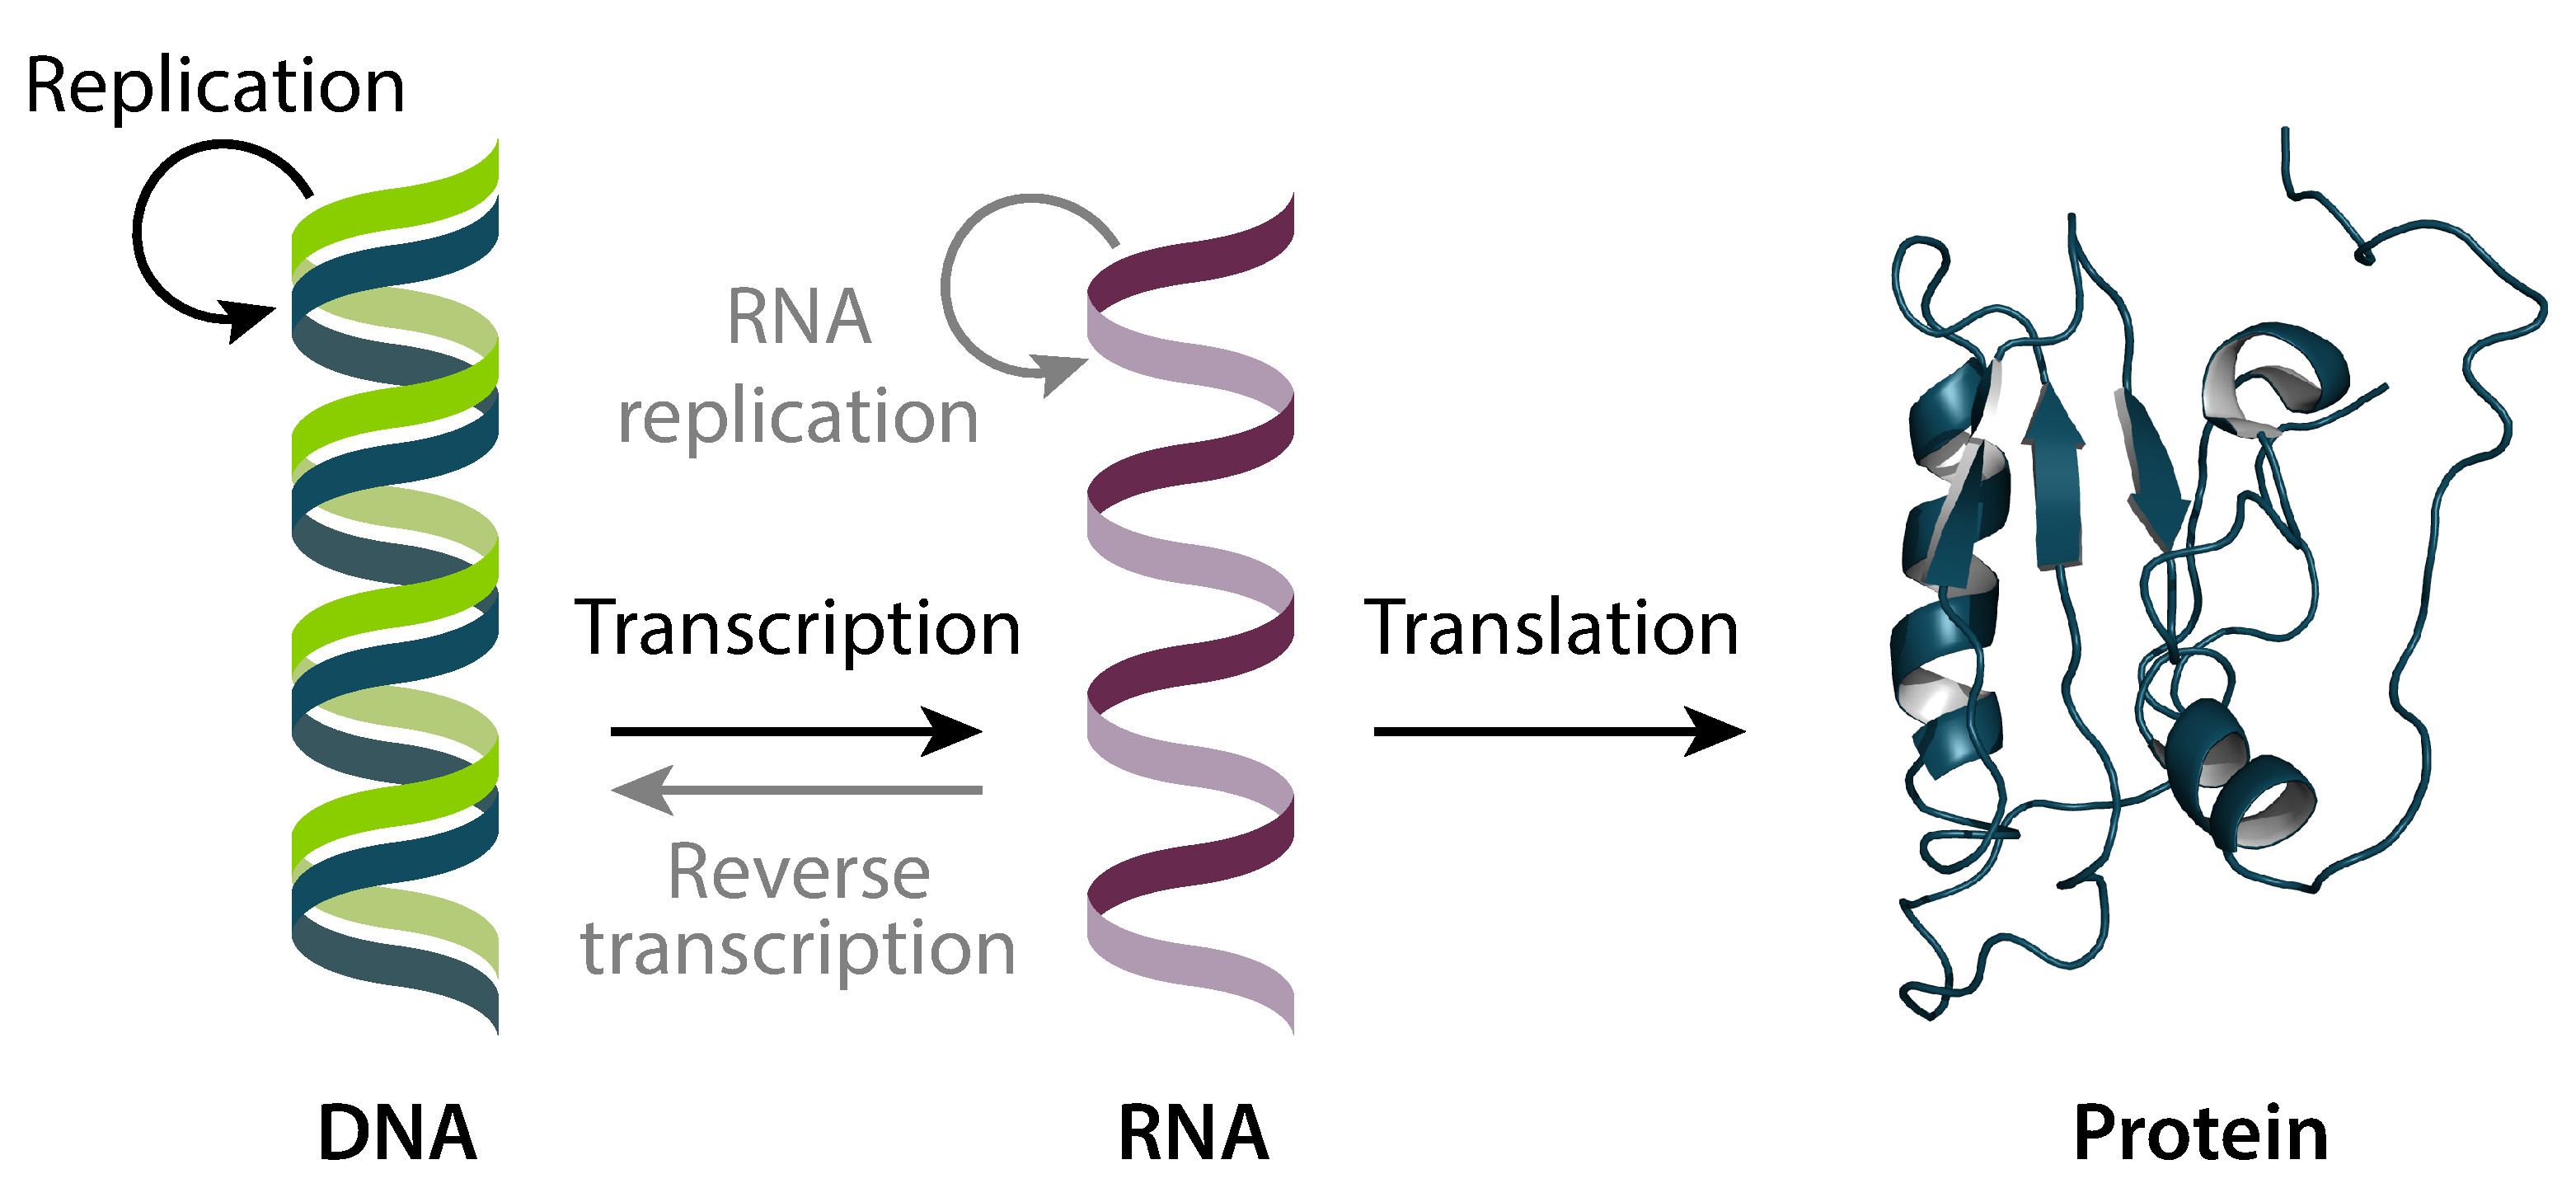
\includegraphics[width=1\linewidth]{figures/central_dogma.pdf}
    \caption{\textbf{Central dogma of molecular biology.} The central dogma of molecular biology states that Deoxiribonucleic Acid (\gls{dna}) replicates itself into more \gls{dna} molecules and it is also transcribed into Ribonucleic Acid (\gls{rna}), which is then translated into proteins. These processes, illustrated with black arrows, constitute the core of the central dogma of molecular biology and the most common flow of \gls{geneexpression}. This dogma has been expanded since its postulation (grey arrows), incorporating processes such as \gls{rna} replication, used by \gls{rna} viruses like poliovirus. Additionally, the Human Immunodeficiency Virus (HIV) utilizes reverse transcription to convert its \gls{rna} genome into \gls{dna}, which is then integrated into the host genome.}
    \label{fig:chapter1:central_dogma}
\end{figure}

\begin{figure}[tbh]
    \centering
    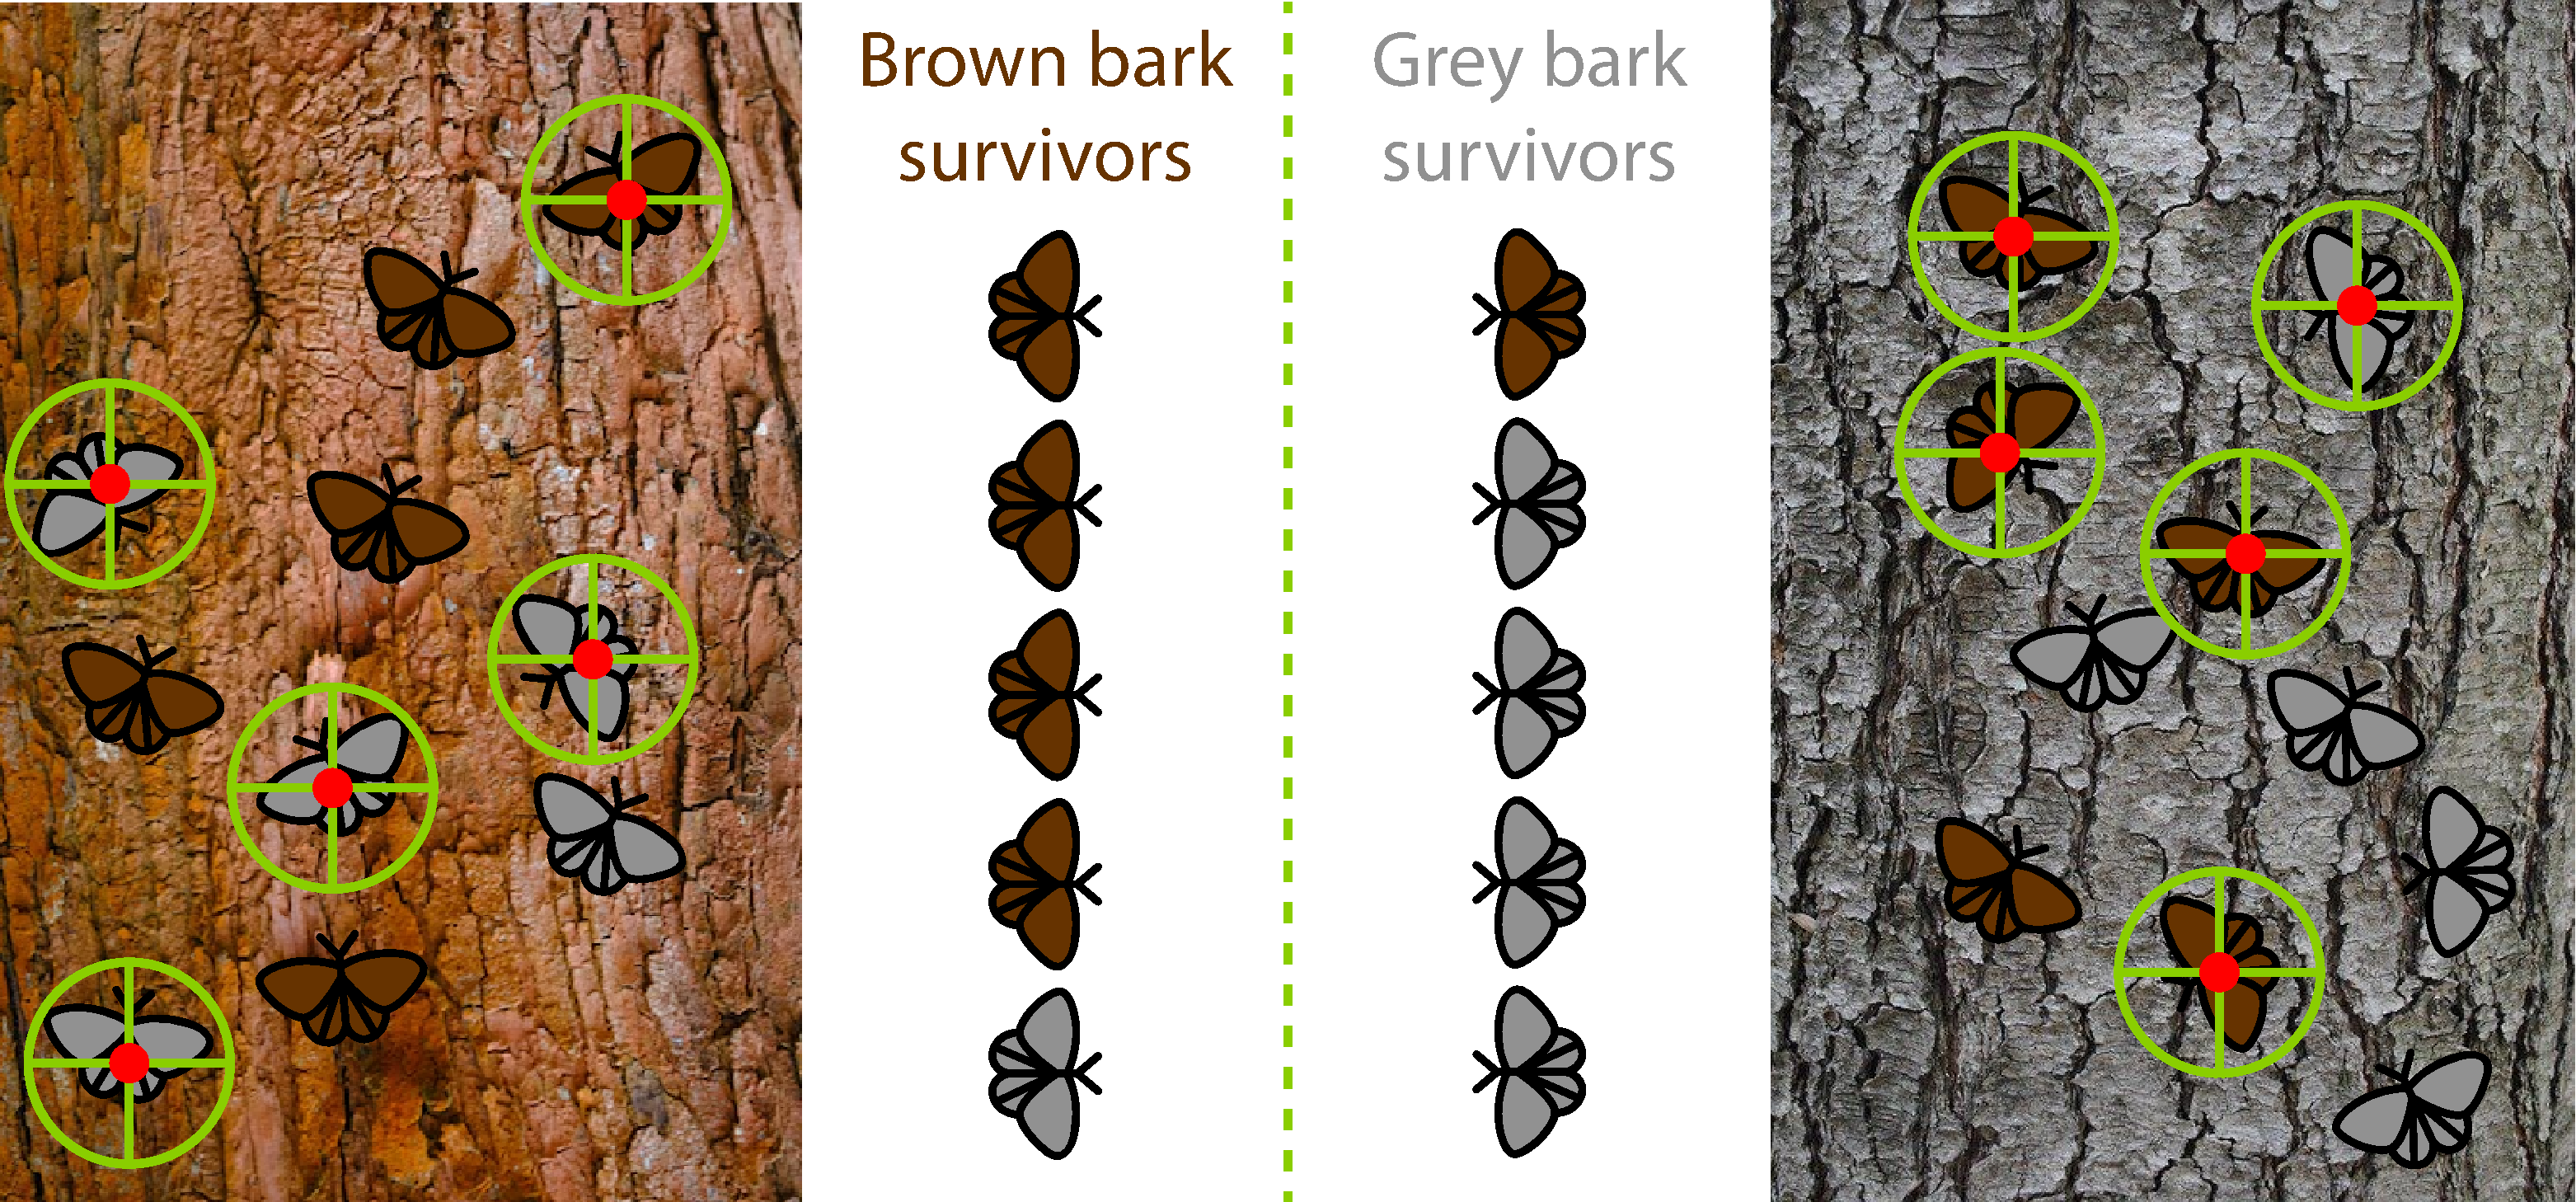
\includegraphics[width=1\linewidth]{figures/evolution_selection.pdf}
    \caption{\textbf{Evolutionary selection in different environments.} A population of moths with two different colours can be differentially selected depending on the environment. In this example, the moths are placed in trees with brown and a gray barks. In the brown bark tree, the gray moths are more visible to predators and are hunted in larger numbers that brown moths, and vice-versa. This results in differential survival rates, which will condition the traits for successful moth generations, selected for higher survival on a given bark colour.}
    \label{fig:chapter1:selection}
\end{figure}


Proteins, as a family of molecules present in living organisms, were formally described in the 19\textsuperscript{th} century \cite{natural_history_museum_library_sur_1838, hartley_origin_1951}. Later, they were characterised as a polypeptide chain \cite{dill_dominant_1990, gutte_peptides_1995}; their \gls{secondarystructure} and stabilisation by \glspl{hydrogenbond} were also described \cite{astbury_molecular_1931, pauling_atomic_1951, pauling_structure_1951}, and the use of \gls{xraycrystallography} crystallography in the 1950s enabled the first elucidation of protein \gls{tertiarystructure} \cite{kendrew_three-dimensional_1958, perutz_structure_1960}. In these early models of tertiary structure, it is noted that some regions are more difficult to elucidate, as quoted: ``If we attempt to trace a single continuous chain throughout the model, we soon run into difficulties and ambiguities, because we must follow it around corners, and it is precisely at corners that the chain must lose the tightly packed configuration which alone makes it visible at this resolution'' \cite{kendrew_three-dimensional_1958}. Even under the cold, dehydrated, and clearly non-native conditions to which proteins are subjected for \gls{xraycrystallography} crystallography \cite{fenwick_integrated_2014}, this was an early observation of protein \gls{dynamics} in structured proteins, illustrated by the spread location of \glspl{electron} in the molecule and consequent low resolution of the elucidated structure.

Protein \gls{dynamics} refer to the various motions and conformational changes that proteins undergo in their functional states. These encompass diverse ranges of motion, from atomic fluctuations and loop movements to large \gls{proteindomain} rearrangements, and time scales from pico-seconds to seconds. Many proteins contain intrinsically \glspl{proteindisorder} regions (\glspl{idr}) or are entirely intrinsically \glspl{proteindisorder} proteins (\glspl{idp}) \cite{tompa_intrinsically_2002, aspromonte_disprot_2024}. Unlike structured proteins, which have a well-defined three-dimensional structure, \glspl{idr} and \glspl{idp} lack a stable tertiary structure under \gls{physiologicalconditions}. These \glspl{proteindisorder} regions feature higher \gls{flexibility}, the ability to adopt diverse \glspl{conformation}, and often play a crucial role in a protein's function, such as \gls{ligand} binding. \Gls{proteindisorder} can also be transient and change according to its environment, such as in fold-upon-binding regions \cite{tsai_folding_1999, wright_linking_2009, fuxreiter_fold_2019}, which only adopt a defined structure during binding processes.

The elucidation of protein tertiary structures with \gls{xraycrystallography} crystallography drove the creation of the Protein Data Bank (PDB) \cite{berman_protein_2012} and nearly caused early research on protein \gls{proteindisorder} and \gls{dynamics} \cite{pauling_theory_1940, jirgensons_classification_1966} to be overshadowed by the determination of defined \glspl{proteinstructure} \cite{bondos_roles_2021}. Since then, protein science has gradually moved its views of \gls{proteinstructure} towards more dynamic models. The once universally accepted lock and key model for enzyme-substrate binding \cite{fischer_einfluss_1894} has transitioned into more dynamic binding models. Once such model is the induced fit model \cite{koshland_application_1958, vasella_glycosidase_2002}, in which the binding site changes \gls{conformation} to fit the substrate or a \glspl{proteindisorder} region folds upon binding \cite{tsai_folding_1999, bonetti_analyzing_2017, delaforge_deciphering_2018, bonetti_how_2018, fuxreiter_fold_2019, robustelli_mechanism_2020}. The other model is the conformational selection model \cite{tsai_structured_2001}, which states that all protein \glspl{conformation} exist in an equilibrium in its unbound state, even the bound \gls{conformation}, and the \gls{ligand} selectively binds to the ones with higher affinity \cite{vogt_conformational_2013, vogt_essential_2014}. 

The discovery of allosterism, the regulation of protein activity by binding to a different region than the active site, showed that such conformational changes can also be mediated by interactions in distant regions of a protein \cite{monod_general_1961, monod_nature_1965}. For example, the kinesin protein, responsible for processes such as intracellular transport, signal transduction, and chromosome movement during cell division, was observed to actively transport vesicles along cell microtubules in a similar motion as how humans walk \cite{vale_molecular_2003, endow_kinesins_2010}. Another example is the discovery of the revolver-like rotation in ATP (Adenosine triphosphate) synthases as a crucial part in transforming a \gls{proton} gradient into energy in the form of ATP \cite{noji_direct_1997}. This is a molecule that acts as the proteins' energy currency which can be ``spent'', hydrolised into ADP (Adenosine diphosphate), for processes that require energy, such as the previously mentioned ``walk'' of the kinesin protein (\figref{fig:chapter1:atp_adp}). Eventually, long-forgotten studies on protein \gls{proteindisorder} regained attention and the dynamic nature of proteins regained relevance.

\begin{figure}[tbh!]
    \centering
    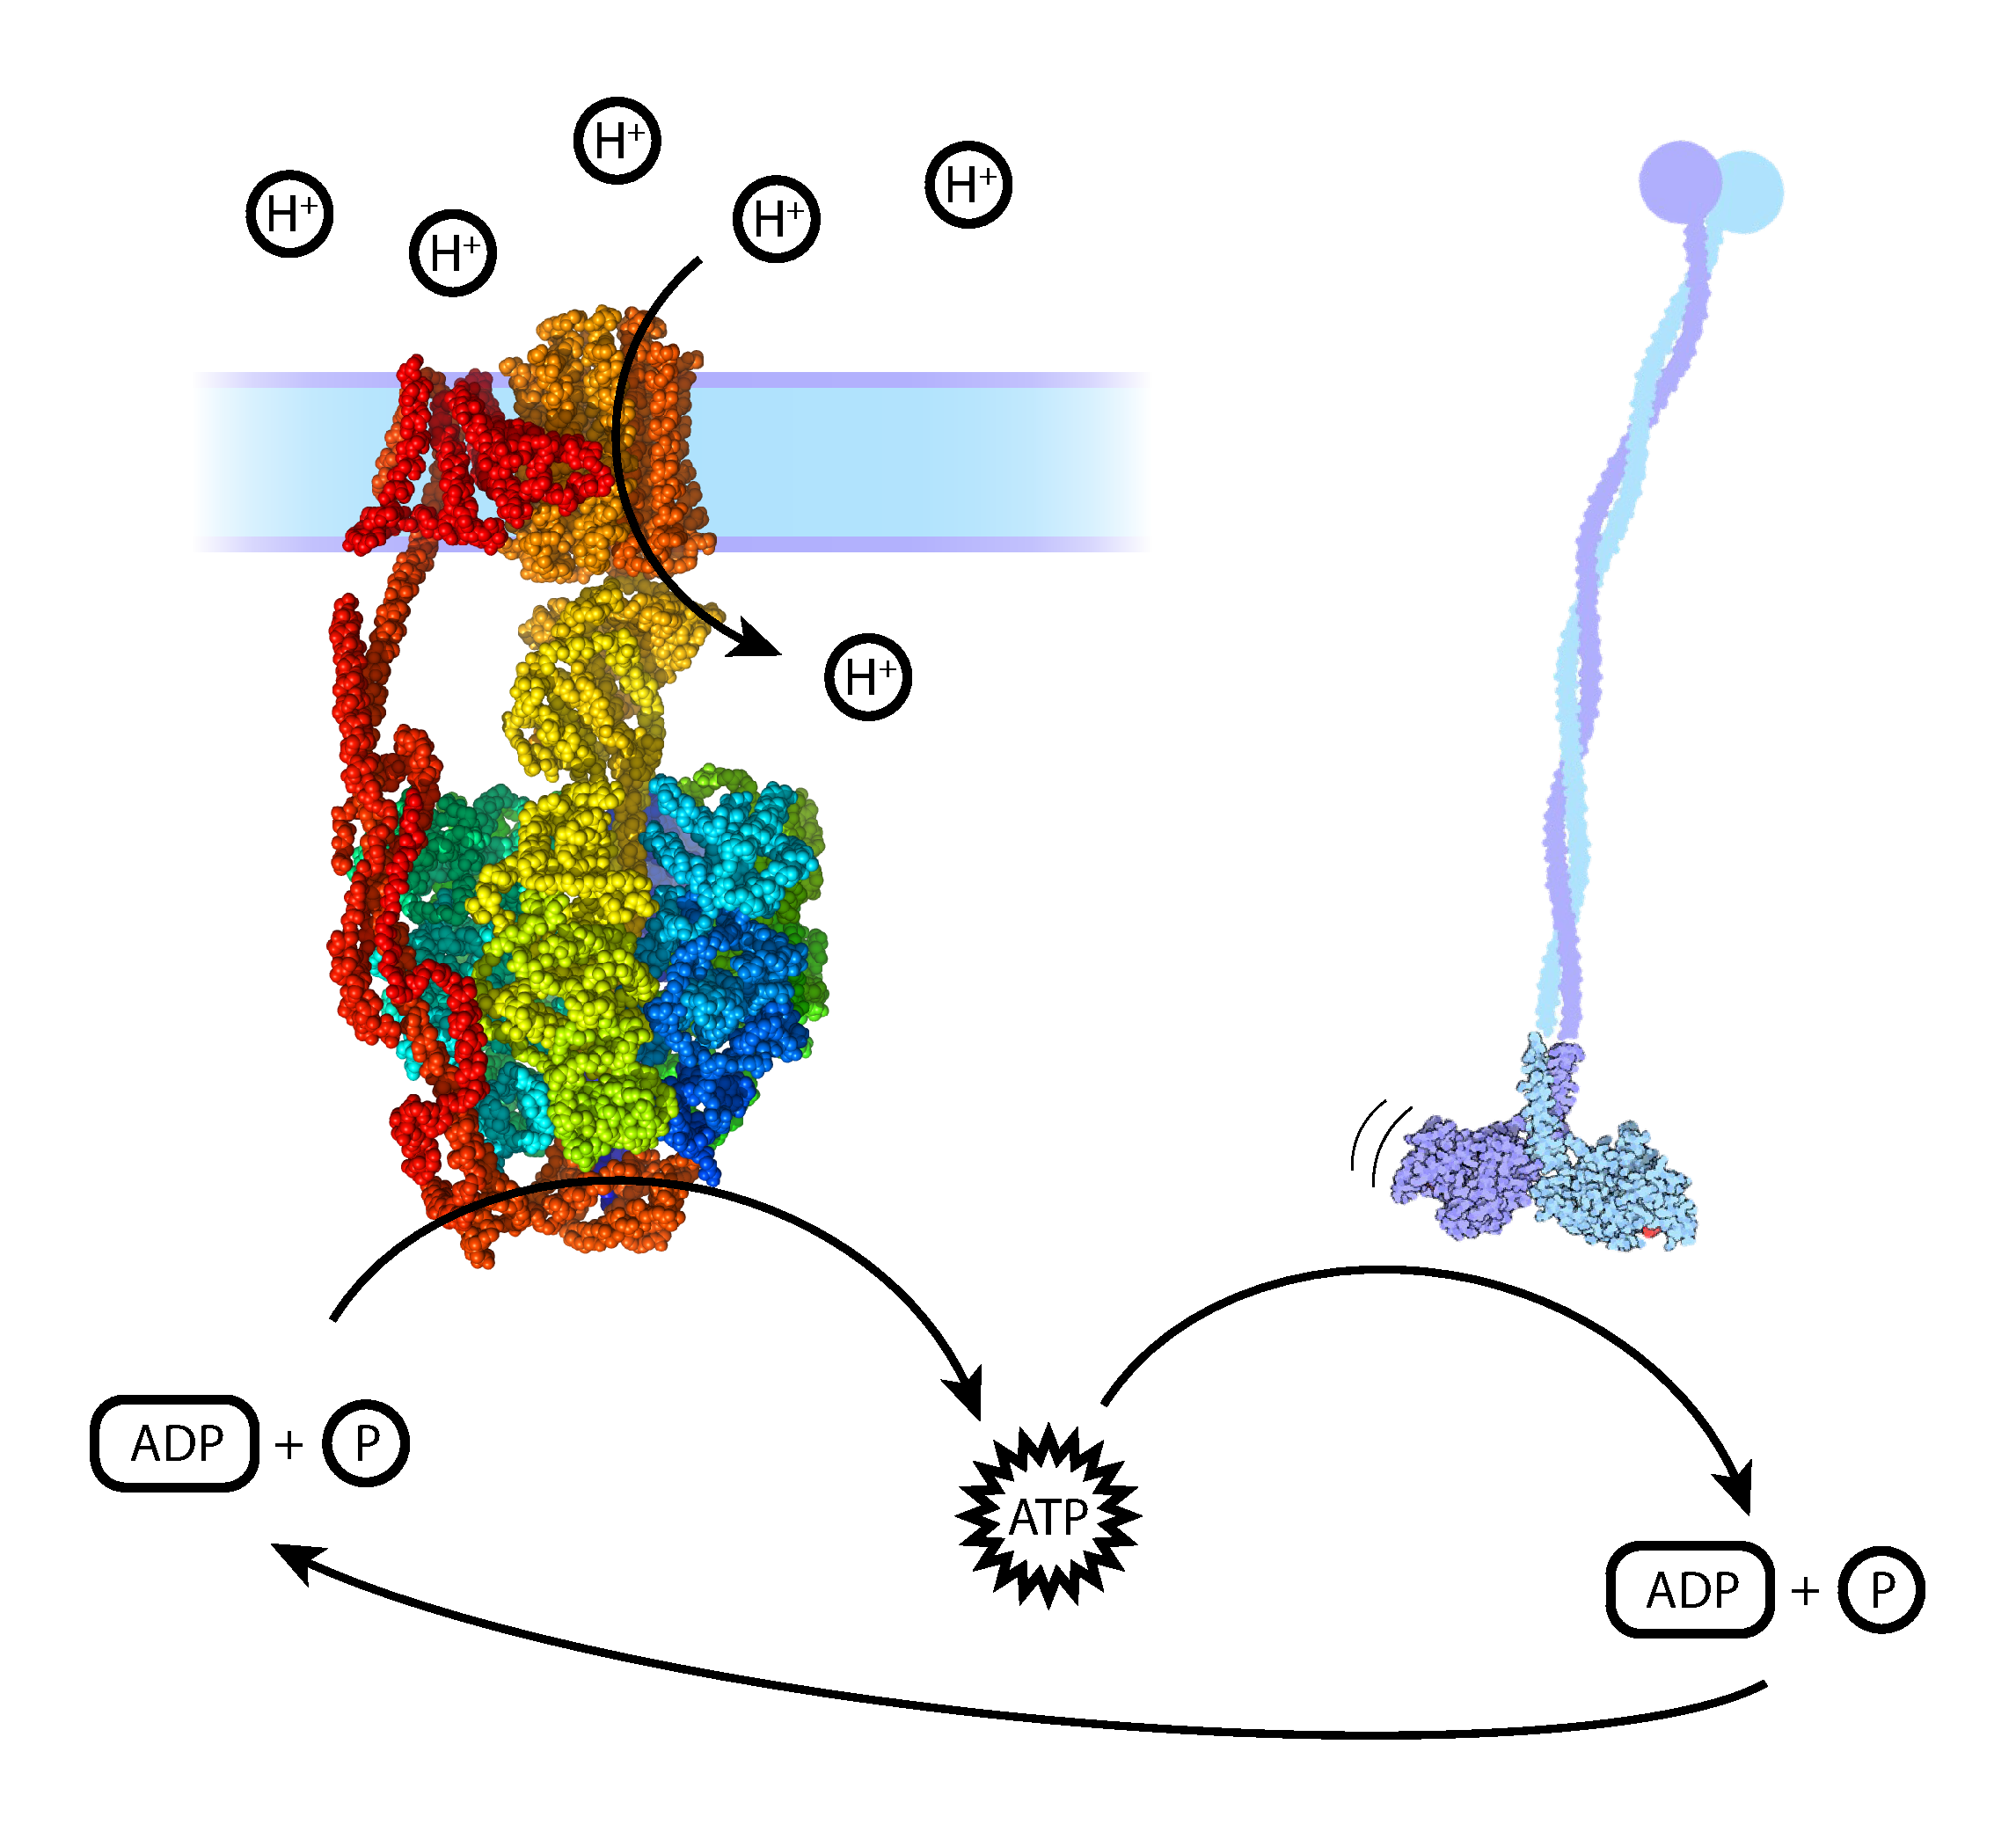
\includegraphics[width=0.8\linewidth]{figures/atp_adp_usage.pdf}
    \caption{\textbf{Synthesis and hydrolisation of ATP.} Mitochondrial ATP synthase (left, PDB-ID 5ARE) uses the \gls{proton} gradient and transport to synthesise ATP from ADP and a phosphate group. The chemical bond that incorporates the new phosphate group is energetically rich, making ATP the cell's energetic currency. This energy can be released through hydrolysis and used for active (i.e., energy-consuming) processes, such as the ``walk'' of the kinesin protein (right, image URL: \url{https://cdn.rcsb.org/pdb101/motm/64/3kin-composite.gif}).}
    \label{fig:chapter1:atp_adp}
\end{figure}


% \section{Protein Structure Fundamentals}
\section{Protein Structural Organisation}

Protein motion is defined by simultaneous effects of endogenous and exogenous factors, some of which we will elaborate in this chapter. One of these is a protein's own structure, which determines its degrees of freedom and stability. The description of \gls{proteinstructure} is hierarchically organised, with each subsequent level describing larger scales of \gls{proteinstructure}. The \gls{primarystructure} of a protein, a protein's lowest structural level, describes it as a polypeptide sequence, a chain of \glspl{aminoacid} bound with peptide bonds. This chain is generally formed by a combination of 20 \glspl{aminoacid} (though non-standard \glspl{aminoacid} lengthen the list), each of them featuring different intrinsic properties (\textit{e.g.} polar, aromatic, hydrophobic...) \cite{neilan_amino_2003}. The peptide bond keeping these \glspl{aminoacid} together is a special kind of bond, as it results in a plane which restricts the trajectory of the polypeptide chain (\figref{fig:chapter1:peptide_bond}), resembling the interleaved rigid-motile-rigid pattern featured in the links of a metal chain. These planes make $\text{C}_{\alpha}$ the only possible flexing point of an \gls{aminoacid} in a poly-peptide chain (besides small variation in $\omega$ angles), and two angles $\phi$ and $\psi$ are defined as the orientation of these planes with respect to $\text{C}_{\alpha}$. 

\begin{figure}[tbh]
    \centering
    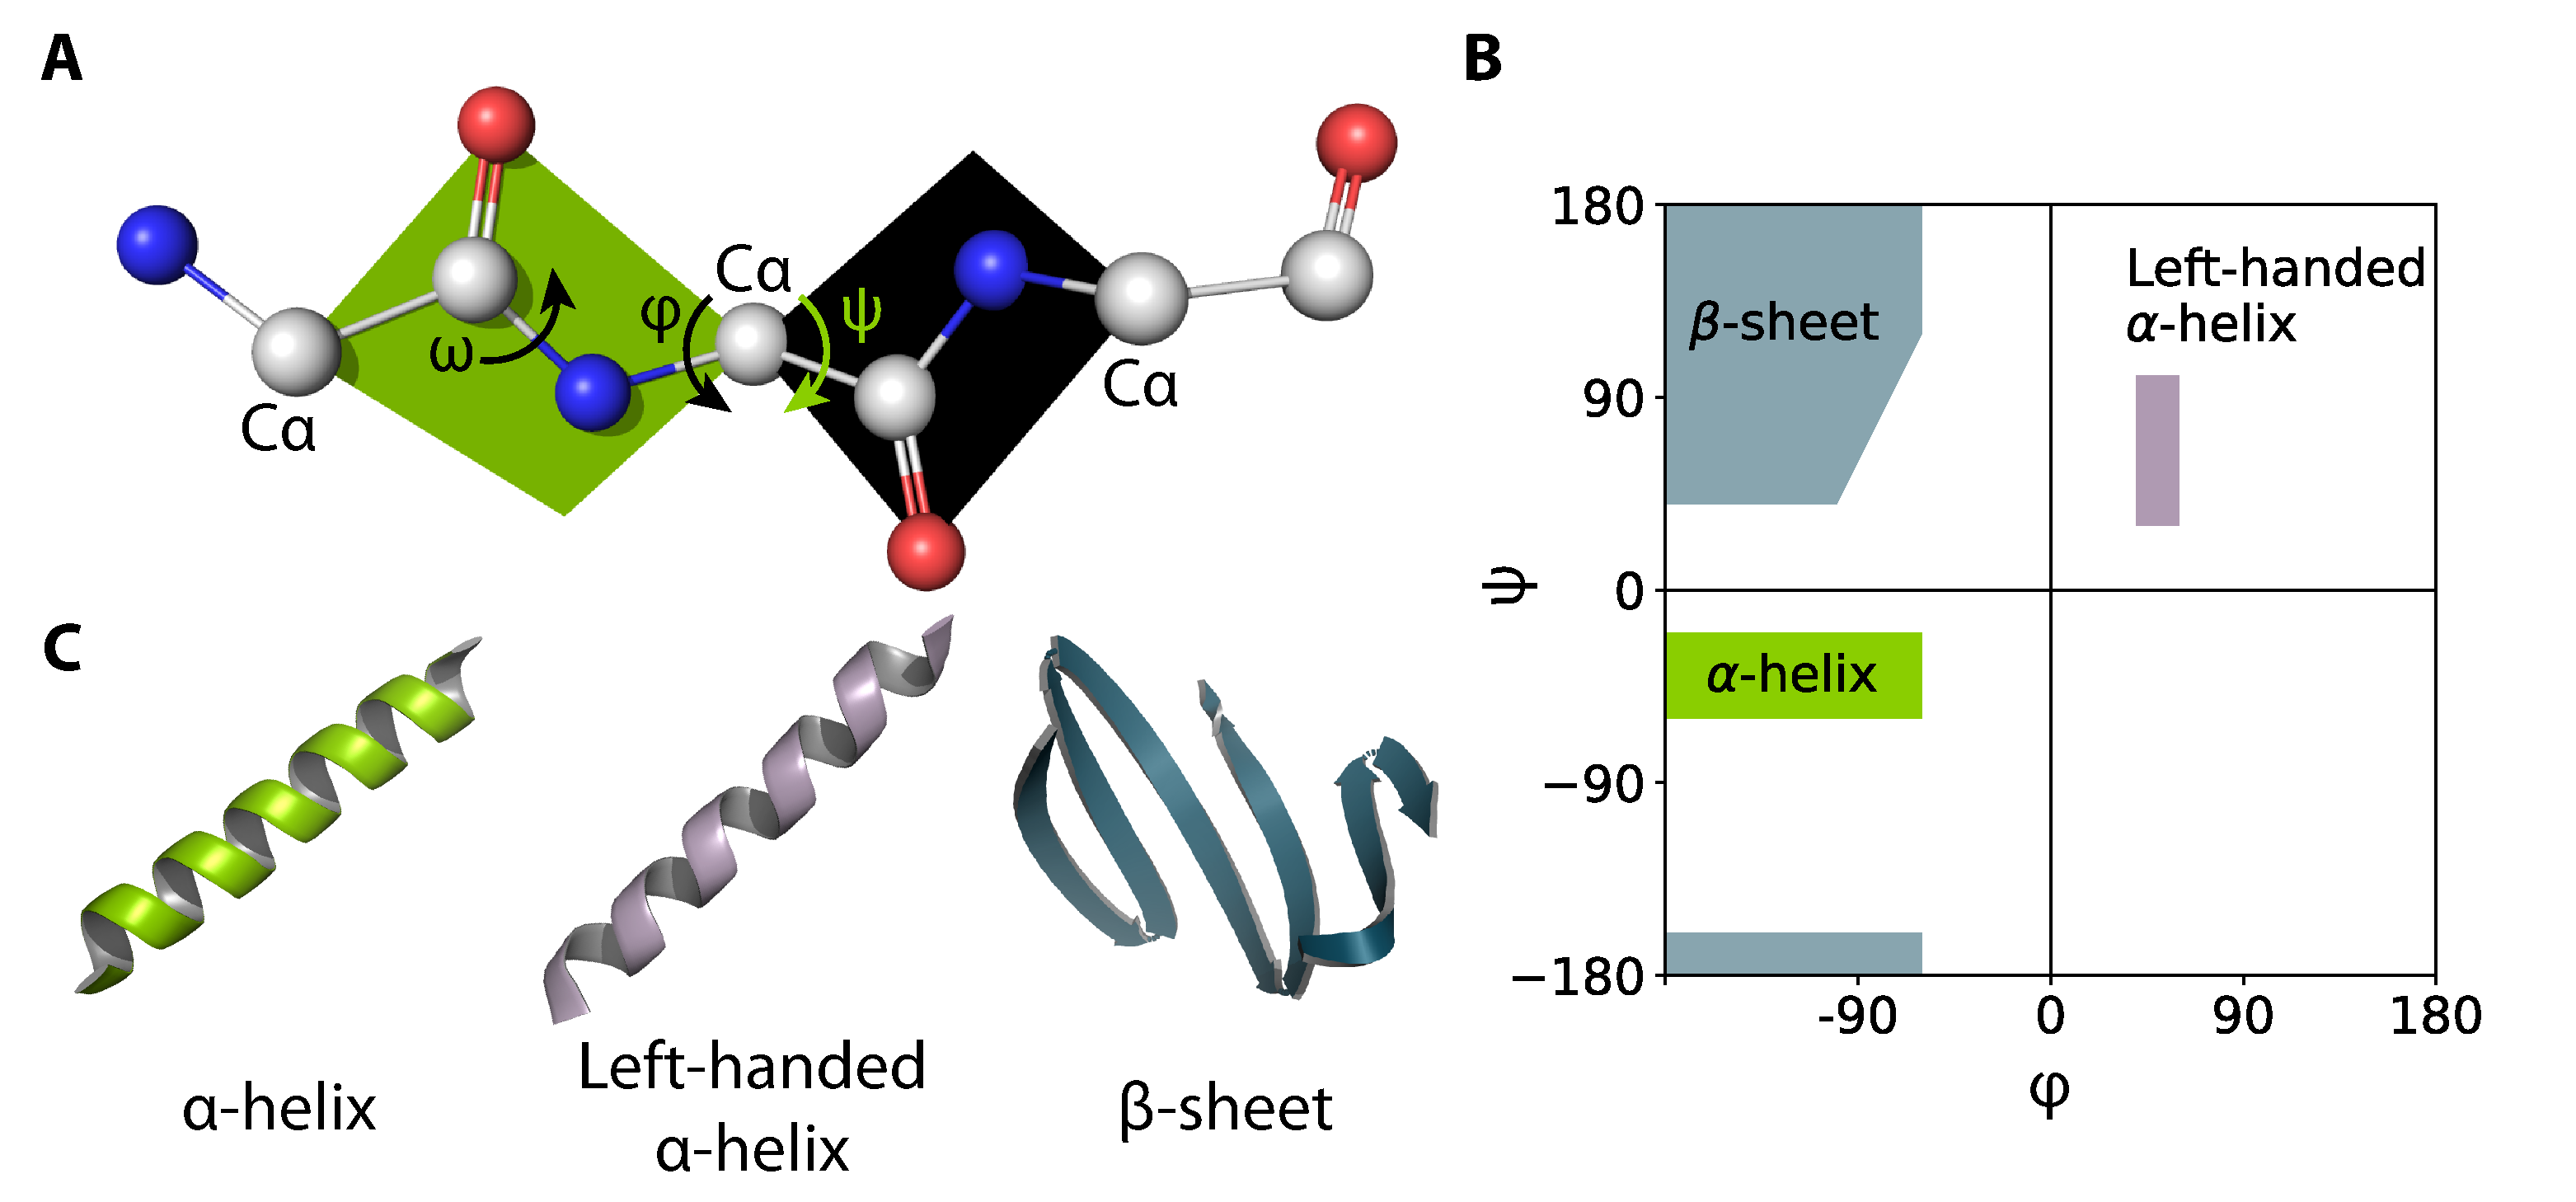
\includegraphics[width=1\linewidth]{figures/peptide_bond_rama.pdf}
    \caption{\textbf{Peptide bond, dihedral angles and their relation to secondary structure.} A) Section of a protein \gls{backbone} centered around the $\text{C}_{\alpha}$ of an \gls{aminoacid}. The peptide bonds between the amino (blue sphere) and the carboxyl (gray and red spheres) groups define a plane, with limited torsion, defined by the omega ($\omega$) angle. These planes' orientation respect to a $\text{C}_{\alpha}$ is described by the phi ($\phi$) and psi ($\psi$) angles. B) The $\phi$ and $\psi$ dihedral angles can be represented in a \gls{ramachandranplot}. This plot represents a torus (doughnut) space where areas can be delimited to represent different types of secondary structures. C) Visualisation of the common secondary structures represented in the \gls{ramachandranplot}.}
    \label{fig:chapter1:peptide_bond}
\end{figure}
 

% Every $\phi$ and $\psi$ angle in every \gls{aminoacid} of the protein determines a sequential path that defines the overall shape of the protein. If a protein's full conformational space (\textit{i.e.} every possible combination of $\phi$ and $\psi$ angles for every \gls{aminoacid}) was explored for a given protein local environment (\textit{e.g.} \gls{physiologicalconditions}, no binding partner, 37$^\circ\mathrm{C}$), a continuum of energy levels could be represented as a multi-dimensional energy surface or landscape \cite{dill_protein_2008}. These energy levels are measured by the \gls{gibbsfreeenergy} \cite{yang_free_2013}, defined as: 


% \begin{equation}
% \label{eq:GibbsFreeEnergy}
% G = H - TS
% \end{equation}

% where \( G \) is the \gls{gibbsfreeenergy}, \( H \) is the \gls{enthalpy} (which represents the total heat content of the system), \( T \) is the absolute temperature (in Kelvin), and \( S \) is the \gls{entropy} (which measures the disorder or randomness in the system). Every change in $\phi$ and $\psi$ angles results in a displacement in the landscape, which carries a change in \gls{entropy} and \gls{enthalpy} and thereby generally a change in \gls{gibbsfreeenergy}. The change of energy associated to change in protein fold is described as follows:

% \begin{equation}
% \label{eq:GibbsFreeEnergyChange}
% \Delta G = \Delta H - T \Delta S
% \end{equation}

% where \(\Delta G\) is the change in \gls{gibbsfreeenergy}, \(\Delta H\) is the change in \gls{enthalpy}, \(T\) is the absolute temperature, and \(\Delta S\) is the change in \gls{entropy} upon folding. At constant temperature (\textit{e.g.} in human \gls{physiologicalconditions}) the \gls{gibbsfreeenergy} is a function of a fold's \gls{enthalpy} and \gls{entropy}. In the context of protein fold, \gls{enthalpy} reduction occurs in events such as the formation of covalent and \glspl{hydrogenbond}, the exclusion of solvent from the system by hydrophobic packing, or aromatic rings stacking \cite{santiago_relation_2010, liu_protein_2012}. \Gls{entropy} refers to the disorder of the system, which is decreased by events such as the exposure of hydrophilic \glspl{aminoacid} to solvent (thereby burying hydrophobic \glspl{aminoacid} in the protein core) freeing the orientation of a protein's surrounding solvent, or the binding to a \gls{ligand} \cite{bonetti_analyzing_2017, bonetti_how_2018}. Proteins aim to reduce their \gls{gibbsfreeenergy}, navigating the energy landscape to reach a \gls{conformation} that represents an energy minimum (\figref{fig:chapter1:landscape}).

\subsection{Thermodynamics view of protein conformation}
Every \(\phi\) and \(\psi\) angle in every amino acid of a protein defines a sequential path that contributes to the overall shape of the protein. The full conformational space of a protein (\textit{i.e.} every possible combination of \(\phi\) and \(\psi\) angles for every amino acid) represents a complex energy landscape that includes both enthalpic and entropic contributions. If we consider a given protein's local environment (\textit{e.g.} physiological conditions, no binding partner, 37°C), this energy landscape can be visualised as a multi-dimensional surface where each point corresponds to a different conformation with a specific Gibbs free energy \cite{dill_protein_2008}.

The Gibbs free energy (\(G\)) of a protein conformation is defined by the equation:

\begin{equation}
\label{eq:GibbsFreeEnergy}
G = H - TS
\end{equation}

where \(H\) is the enthalpy (the total heat content of the system), \(T\) is the absolute temperature in Kelvin, and \(S\) is the entropy (which measures the disorder or randomness in the system) \cite{yang_free_2013}. 

The entropic contribution to the Gibbs free energy, which is related to the number of microstates adopted by the system, including surrounding water molecules, is difficult to capture. For example, the Gibbs free energy of proteins that adopt a single unique conformation with minimal internal entropy will decrease during the folding process, with the reduction in entropy compensated by enthalpic factors such as hydrogen bonding. Therefore, their Gibbs free energy can be approximated to their enthalpy, such as:

\begin{equation}
\label{eq:GibbsFreeEnergy_only_enthalpy}
G \approx H
\end{equation}


% Considering a folded protein that can only adopt a single conformation, such a protein would essentially have zero configurational entropy, as the system is restricted to a single microstate. Without the ability to explore multiple conformations, the protein lacks the structural variability that contributes to entropy. Some other forms of entropy could still have minor contributions on the system, such as solvent-related entropy (\textit{e.g.} changes in the orientation of water molecules surrounding the protein) or vibrational entropy (\textit{e.g.} compression and stretching of chemical bonds). Nevertheless, the overall entropy of the system would be significantly reduced with no contribution from conformational freedom. Therefore, its Gibbs free energy can be approximated to its enthalpy, such as:

% \begin{equation}
% \label{eq:GibbsFreeEnergy_only_enthalpy}
% G \approx H
% \end{equation}

Changes in this system's Gibbs free energy are therefore mostly due to changes in the system's enthalpy. Enthalplic changes can still occur in fixed conformations, for example by the formation of chemical bonds or by the post-translational modification of residues, described by:

\begin{equation}
\label{eq:GibbsFreeEnergy_only_enthalpy_change}
\Delta G \approx \Delta H
\end{equation}

where \(\Delta G\) is the change in Gibbs free energy, \(\Delta H\) is the change in enthalpy. Note that the approximation, rather than equality, in equations \ref{eq:GibbsFreeEnergy_only_enthalpy} and \ref{eq:GibbsFreeEnergy_only_enthalpy_change} allocates for the small contributions to the system of non-configurational entropies.

On the other hand, the thermodynamically most stable state of intrinsically disordered proteins, which do not have a unique fold, will be rather driven by entropic effects and multiple conformations. The overall role of water molecules in this energy landscape is very difficult to capture and at the moment understudied.

For proteins with flexible structures, changes in \(\phi\) and \(\psi\) angles lead to different protein conformations, which are associated with changes in both enthalpy and entropy, thereby altering the Gibbs free energy of the system. The change in Gibbs free energy associated with a transition between different protein conformations, such as folding, is described by:

\begin{equation}
\label{eq:GibbsFreeEnergyChange}
\Delta G = \Delta H - T \Delta S
\end{equation}

where \(\Delta G\) is the change in Gibbs free energy, \(\Delta H\) is the change in enthalpy, and \(\Delta S\) is the change in entropy upon folding or unfolding. At constant temperature (e.g. in human physiological conditions), the Gibbs free energy reflects the balance between enthalpy and entropy changes as the protein explores its conformational space.

\subsection{Thermodynamics of protein folding}
During protein folding, various interactions like hydrogen bonds, hydrophobic effects, and van der Waals forces contribute to a reduction in enthalpy by stabilising specific conformations \cite{santiago_relation_2010, liu_protein_2012}. Simultaneously, the folding process reduces the protein’s entropy due to the decreased conformational freedom of the polypeptide chain. However, this entropic cost can be offset by an increase in the entropy of the surrounding solvent as hydrophobic groups are buried away from water, freeing water molecules that were previously structured around these groups, oriented in a polar manner \cite{bonetti_analyzing_2017, bonetti_how_2018}.

Proteins naturally fold to minimise their Gibbs free energy, finding a conformation that represents an energy minimum, which is the most stable state under given conditions (\figref{fig:chapter1:landscape}).


\begin{figure}[tbh!]
    \centering
    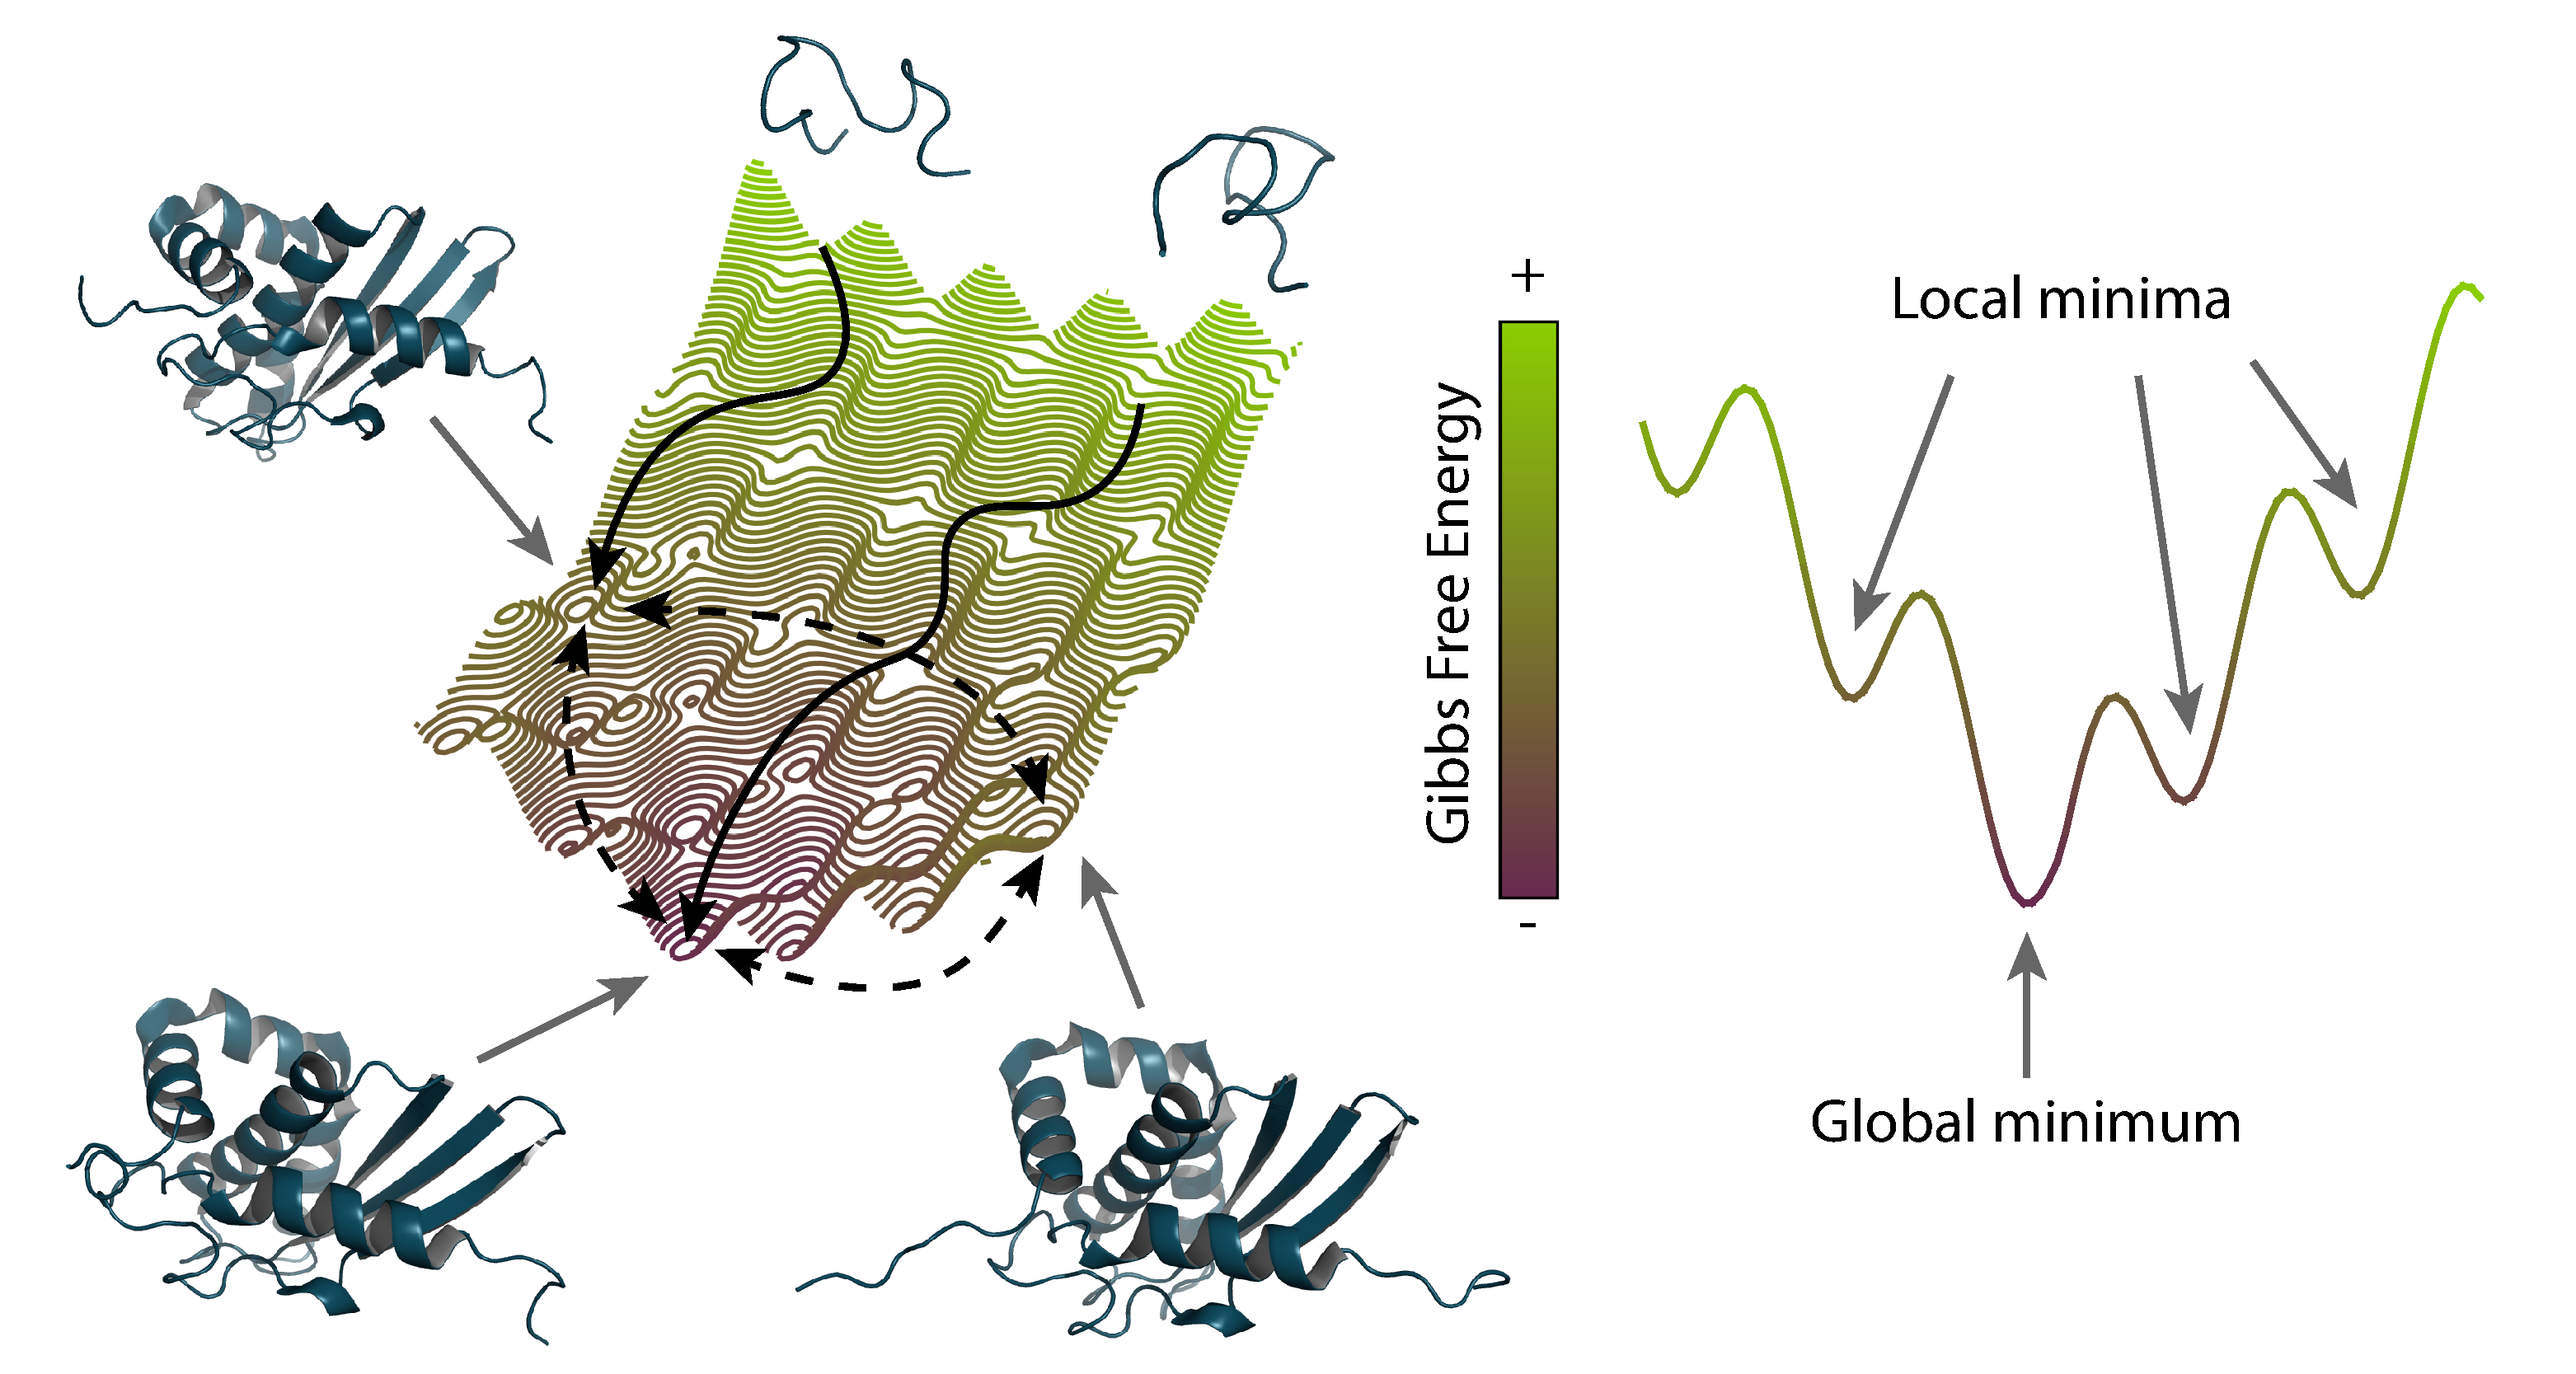
\includegraphics[width=1\linewidth]{figures/energy_landscape.pdf}
    \caption{\textbf{\gls{gibbsfreeenergy} landscape in 3D and 2D representations.} A protein acquires a fold by finding lower-energy states on the \gls{gibbsfreeenergy} landscape. On the left, two different paths to fold (solid black lines) are illustrated on a 3D representation of the landscape, where both paths reach an energy minimum state. The rightmost path reaches the global minimum, while the leftmost stays in a local minimum. These minima are more clearly visualised in the 2D representation on the right side of the figure. This landscape shows the thermodynamic stability of different \glspl{conformation} that lie in \glspl{localminima} energy states. Transitions between these conformations, such as moving from a local minimum to the global minimum, require overcoming energy barriers (peaks in the landscape), which is a kinetic process that depends on the rate at which these barriers can be crossed. PDB ID: 2M5H \cite{ouyang_solution_2013} (diverse conformers from the \gls{nmr} ensemble).}
    \label{fig:chapter1:landscape}
\end{figure}

The simplest spatial structural description of a protein is the secondary structure of its regions. Secondary structures are defined by their \gls{hydrogenbond} stabilisation patterns and their \glspl{aminoacid}' $\phi$ and $\psi$ dihedral angles (\figref{fig:chapter1:peptide_bond}). Proteins further reduce their \gls{gibbsfreeenergy} by folding and adopting their tertiary structure (\textit{i.e.} their overall monomeric \gls{conformation}). In some cases, proteins are composed of multiple sub-units or chains (\textit{e.g.} Mitochondrial ATP synthase in \figref{fig:chapter1:atp_adp}, coloured by chain). These proteins also feature a \gls{quaternarystructure}, which describes how these sub-units bind together to adopt a thermodynamically-favourable \gls{conformation}.

\subsection{The Folding Process}
The process followed by a protein to acquire a functional \gls{conformation} is called its folding process. This process occurs as a complex interaction of entropic and enthalpic elements, described in this section, such as solvent effects, presence of \gls{electrostaticinteractions}, or interaction with other proteins. These elements take place simultaneously and compete with or assist each other at different stages \cite{onuchic_theory_2004}. The effects of these elements can be permanent in a protein's final \gls{conformation} (\textit{e.g.} formation of \glspl{hydrogenbond} that define a secondary structure element, formation of disulphide bonds between cysteine \glspl{aminoacid}, appending post-translational modifications to the \glspl{aminoacid}, or the binding of sub-units in a multimeric protein), or be transient and employed to overcome an energy barrier and further descend in the \gls{gibbsfreeenergy} landscape (\textit{e.g.} binding of chaperones \cite{dandage_classification_2015, balchin_recent_2020, lu_energy_2021} or temporary co-factors \cite{wittung-stafshede_role_2002, wilson_role_2004, bushmarina_cofactor_2006}). A \gls{foldingpath} is defined as a result of these elements' interaction, which results in a descent in the \gls{gibbsfreeenergy} landscape to \glspl{conformation} with lower energy levels. As proteins adopt a conformation, even proteins that will later remain in a single unique conformation will experience a descent in Gibbs free energy during the folding process. These also experience entropic effects because they are not yet restricted to a single microstate during the folding process and can therefore transition between them. The number of allowed microstates narrows as the folding process progresses, in some cases up to a single conformation.


The folding of a protein can be divided into the acquisition of both local and global \glspl{conformation}. The local \gls{conformation} refers to the spatial arrangement of the protein’s \gls{aminoacid} sequence within short segments, including secondary structures and \glspl{foldon}. \Glspl{foldon} are regions of the protein that fold quasi-independently, with minimal \glspl{foldingfrustration} (i.e., their folding process does not significantly affect the folding of other regions) \cite{panchenko_foldons_1996, maity_protein_2005, englander_nature_2014}. The interactions between all elements of a protein’s local \gls{conformation} contribute to the formation of its global \gls{conformation}, which is the protein's overall three-dimensional structure at a given time.

Generally, the \gls{nativefold} of a protein is defined as the lowest energy point of this landscape under \gls{physiologicalconditions}. This landscape's topology is rugged funnel-shaped, biased towards the \gls{nativefold} \cite{onuchic_theory_2004}, with \glspl{localminima} that represent relatively stable \glspl{conformation} that a protein can adopt \cite{tsai_structured_2001} (\figref{fig:chapter1:landscape}). Later in this thesis, it will be posited that \gls{proteinstructure} is better explained as a continuum of allowed \glspl{conformation}.


\section{Experimental Study of Protein Motion}

\subsection{Molecular Biology and Microscopy Methods}

Different time scales and magnitudes of protein motions require different methods for their study (\figref{fig:chapter1:timescale}). At the largest magnitudes of motions, there is a variety of proteins capable of large molecular motions, essentially molecular motors responsible for large molecular motions \cite{schliwa_molecular_2003}. Some of these largest motions can be identified with creative molecular biology techniques, like the linking of larger and/or fluorescent molecules to mobile regions of a protein, in combination with \gls{microscopy}. These large protein motions are often responsible for crucial cellular processes, such as mitochondrial respiration with the previously mentioned ATP synthase (\figref{fig:chapter1:synthase_rotation}) \cite{noji_direct_1997, sambongi_mechanical_1999, hirono-hara_pause_2001}, transport of cargo in vesicles along microtubules with the hand-over-hand walk of Kinesins \cite{yildiz_kinesin_2004}, or the separation of chromosomes during cell division \cite{sawin_motor_1991, schliwa_molecular_2003}.

\begin{figure}[tbh!]
    \centering
    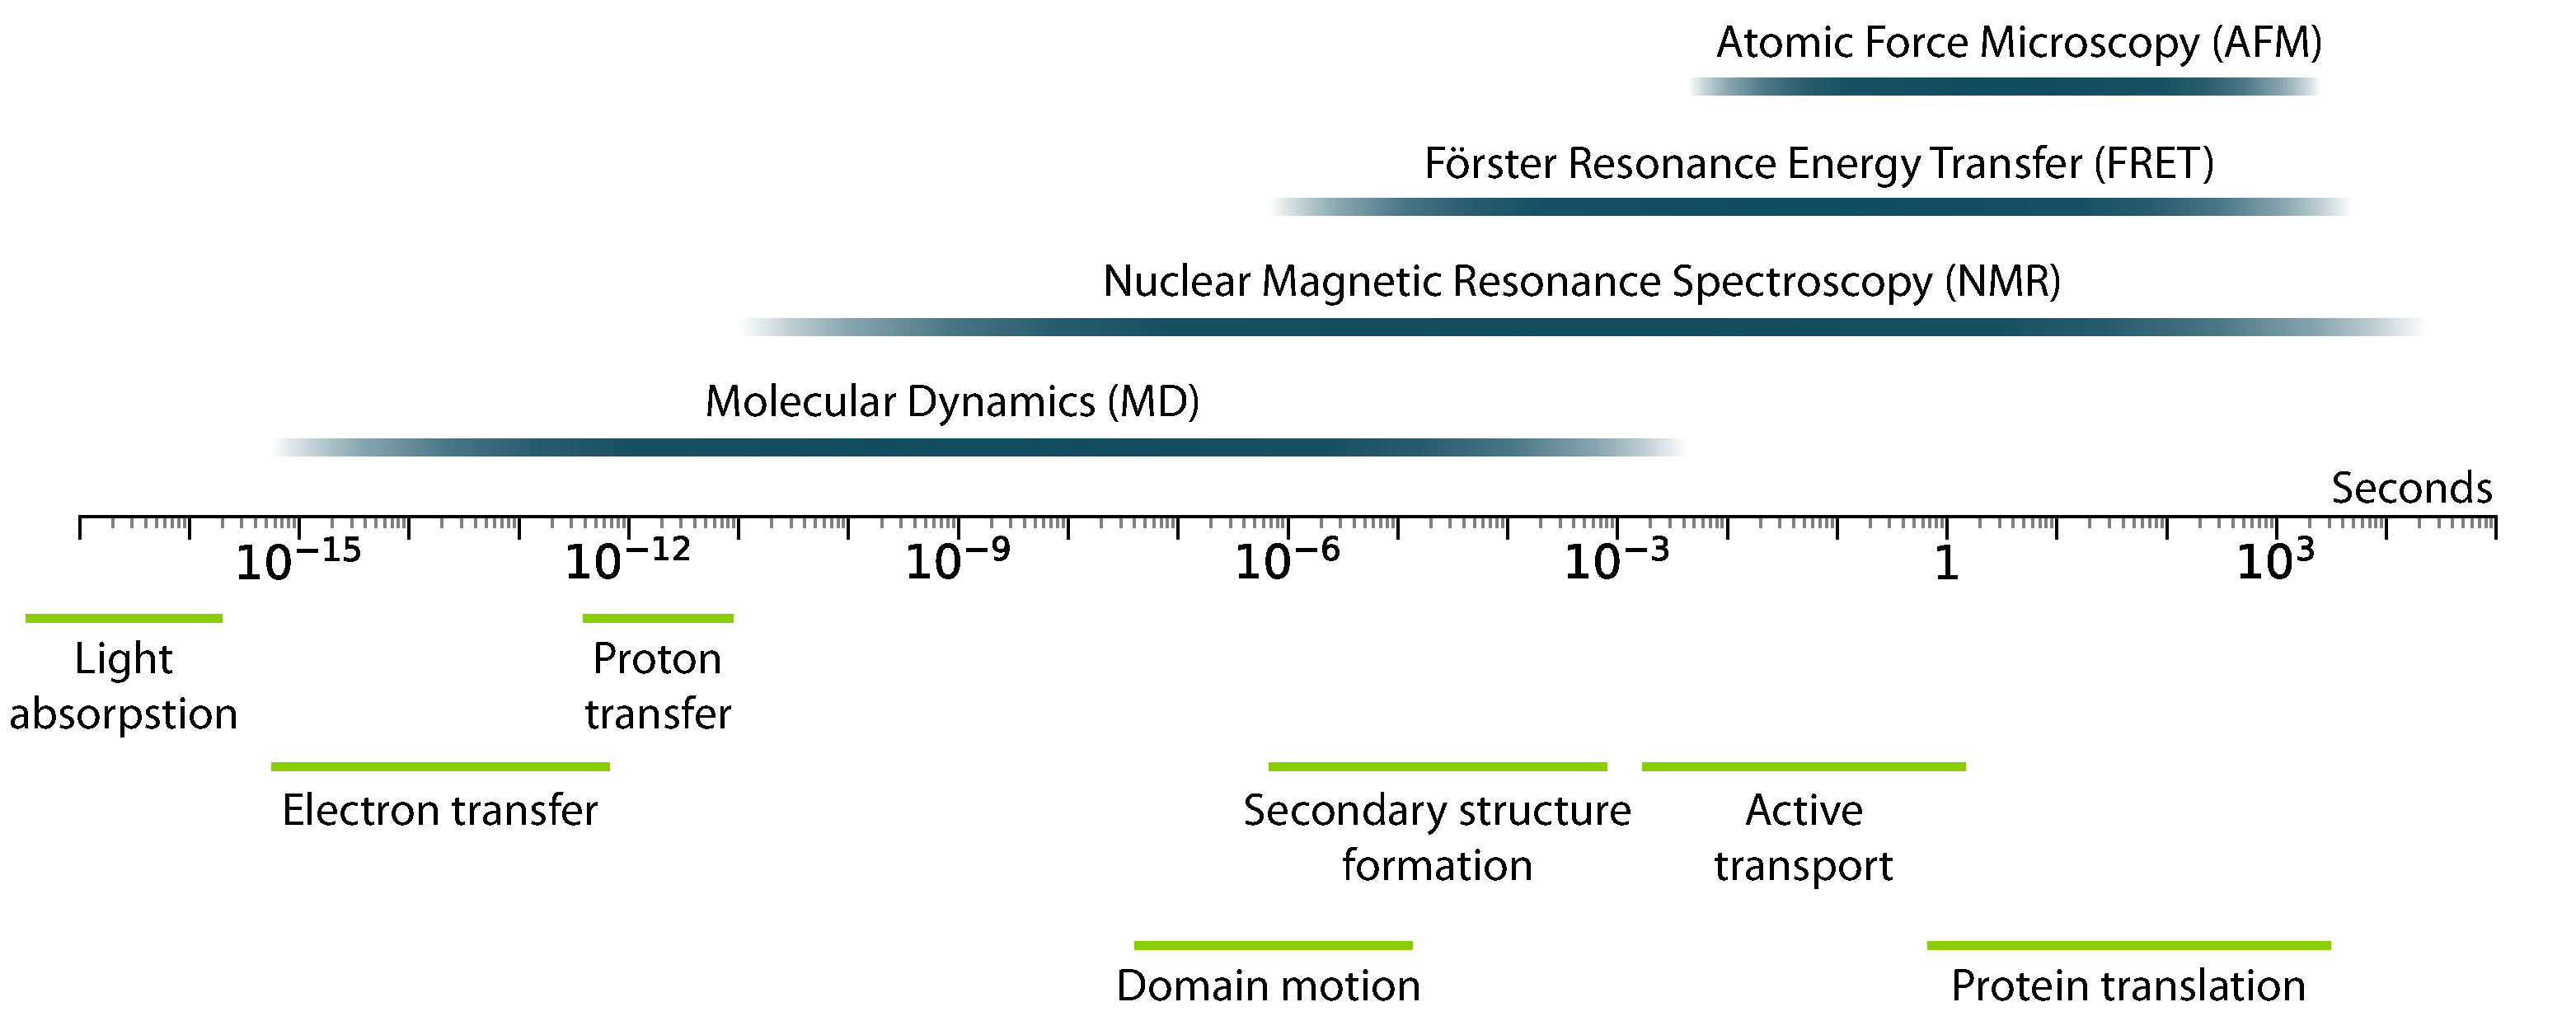
\includegraphics[width=1\linewidth]{figures/timescale_dynamics.pdf}
    \caption{\textbf{Time scale for protein \gls{dynamics} methods compared to physical and biological processes.} Diverse methods to study protein \gls{dynamics} (top) and their time resolution are illustrated with the time-scale of physical and biological processes (bottom). Adapted from Fig. 1 in \cite{ode_molecular_2012}).}
    \label{fig:chapter1:timescale}
\end{figure}

\begin{figure}[tbh!]
    \centering
    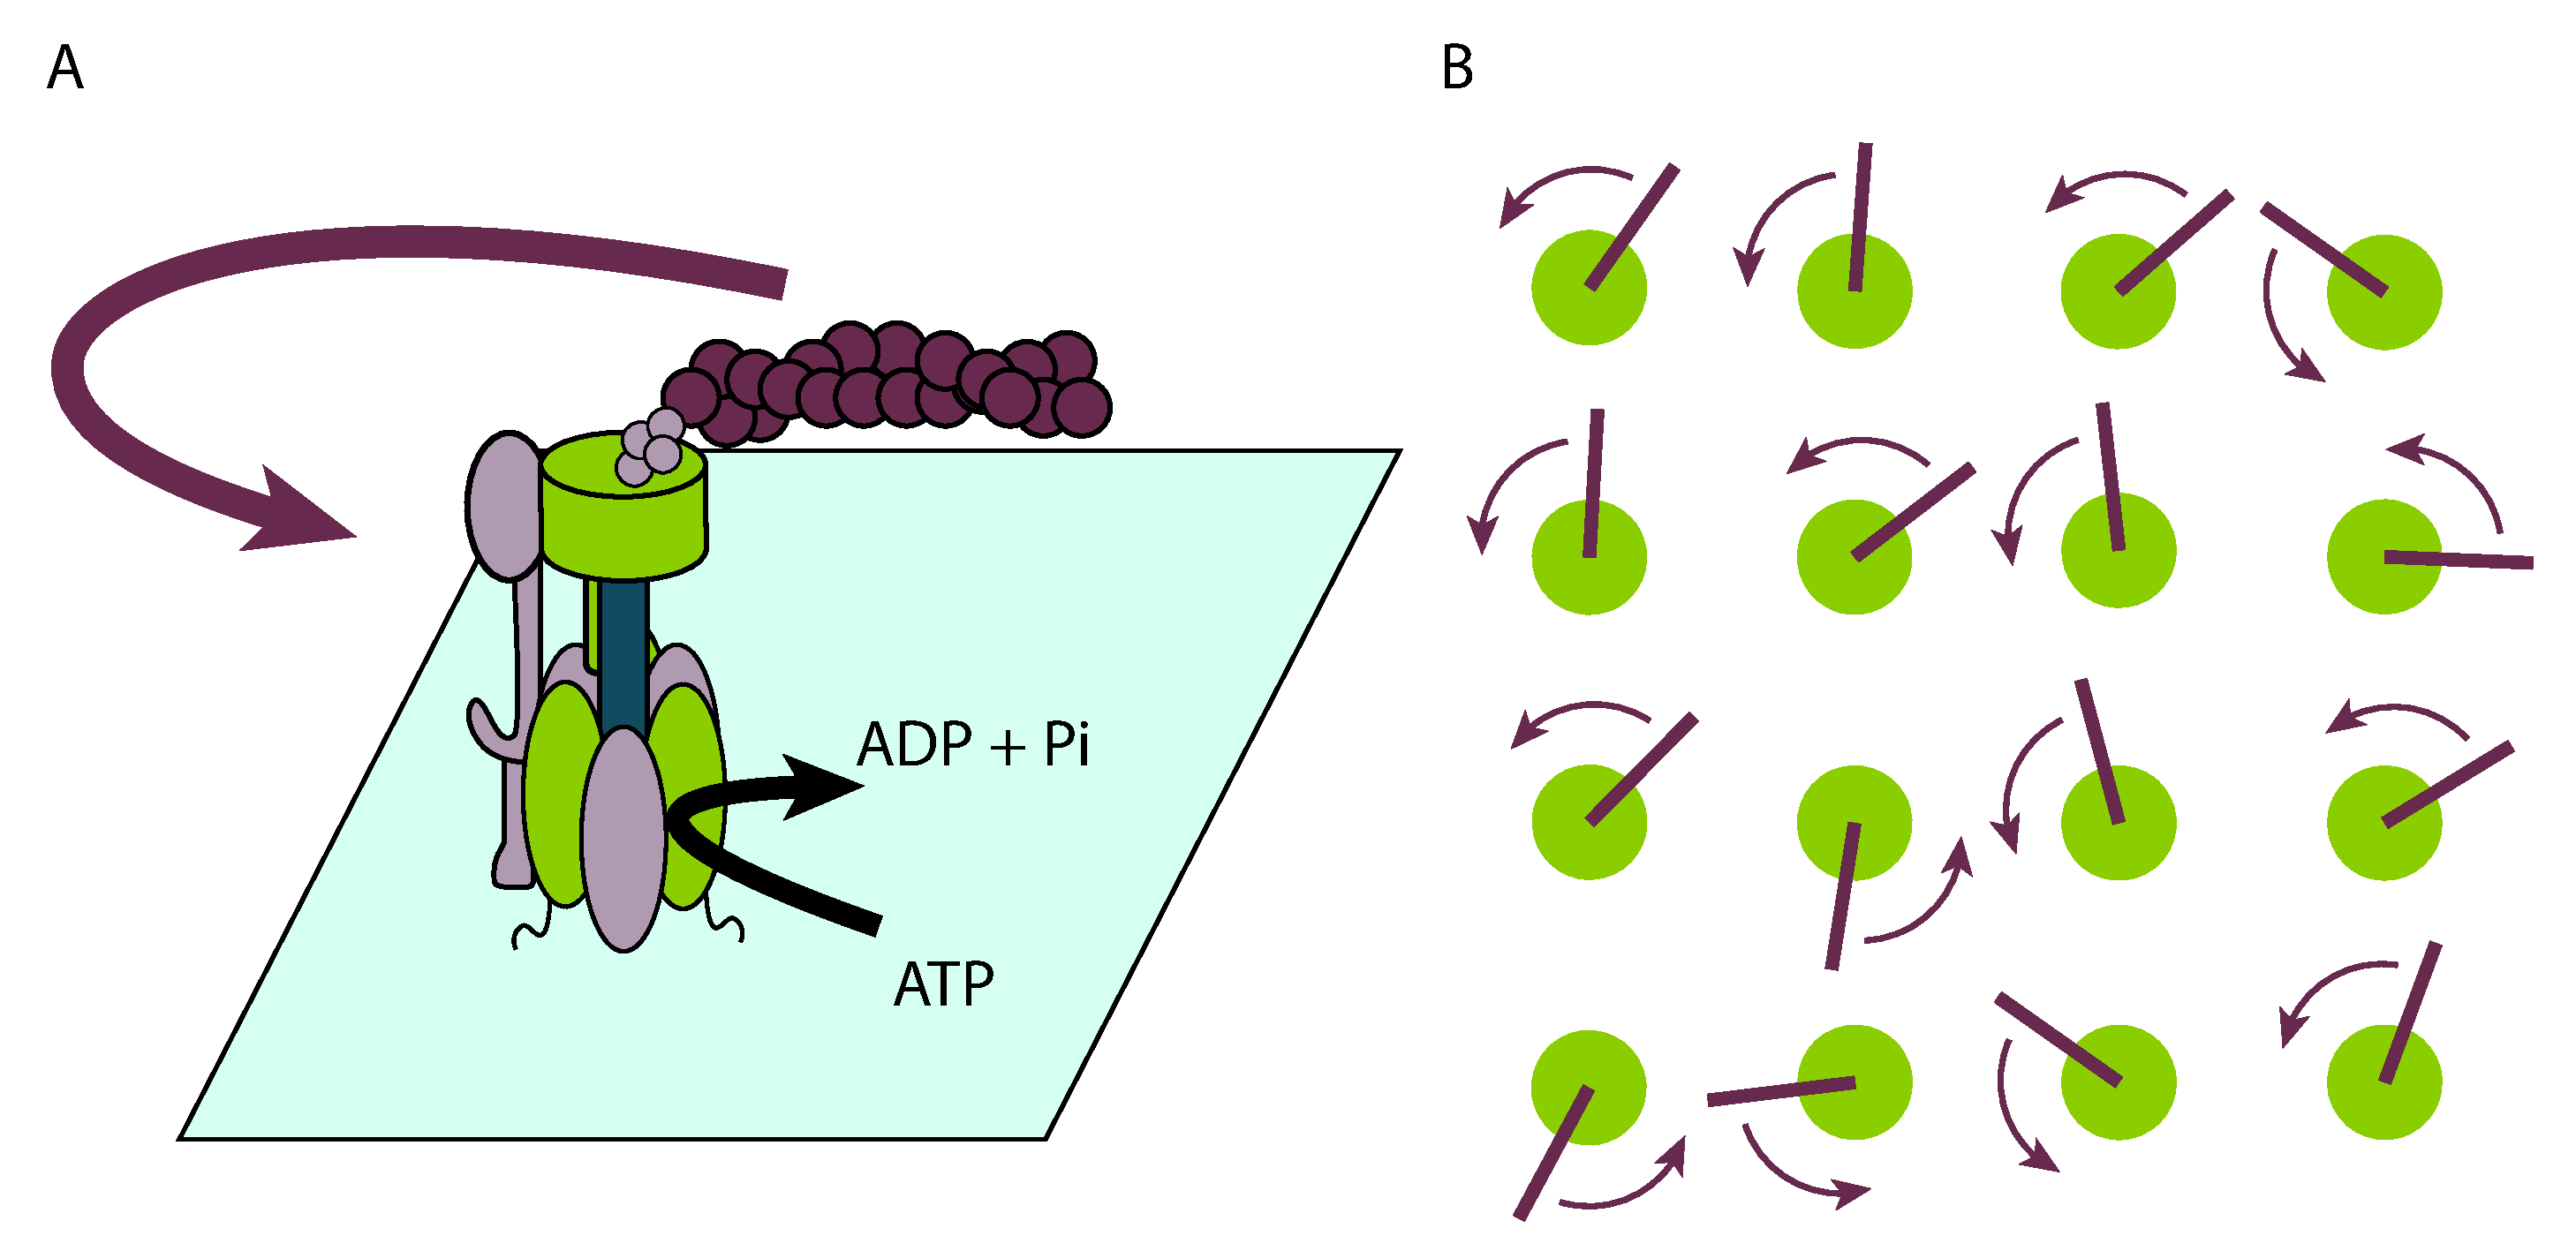
\includegraphics[width=1\linewidth]{figures/experimental_techniques_microscopy.pdf}
    \caption{\textbf{Experimental set-up to observe mechanical rotation of ATP synthase.} A) ATP synthase fixed to a surface and with an actin filament attached to its top sub-unit (F0 sub-unit, not labeled). When ATP is added to the environment, this enzyme hydrolyses it into ADP and a Phosphate group (Pi), which causes the top sub-unit to rotate (Image adapted from \cite{sambongi_mechanical_1999}). B) Top view (\gls{microscopy} perspective) of multiple labeled ATP synthase enzymes fixed to a surface and exposed to ATP. The actin filaments rotate as a result of ATP hydrolisation. This movement can be observed with \gls{microscopy} techniques.}
    \label{fig:chapter1:synthase_rotation}
\end{figure}


Similarly, techniques such as Förster Resonance Energy Transfer (FRET) or their single-molecule variant (smFRET) allow the measurement of proximity between molecules or two regions of the same molecule over a period of time. This technique works by attaching two fluorescent labels to the interacting regions or molecules (\figref{fig:chapter1:fret}). Each label has characteristic light excitation and emission wavelength (light colour) ranges (absorbs energy of light with colour X and emits colour Y), where the emission wavelength range of one bead overlaps with the excitation range for the second. When both beads are isolated and exposed to light in the excitation wavelength of the first label, the emission wavelength of the second label will not be observed. If these labels are in close proximity, \textcolor{red}{the energy obtained from exciting the first label is transferred to the second label. Then, the latter will emit light in its emission wavelength, thus indicating proximity. This method's ability to measure molecular distances makes it suitable to study \glspl{ppi} and conformational changes \cite{truong_use_2001, heyduk_measuring_2002}.}
% the energy from the first label's emission will be absorbed by the second, which will emit light in its emission wavelength, thus indicating proximity. 
% This method can be employed, for instance, to identify protein conformational changes or \glspl{ppi} \cite{truong_use_2001, heyduk_measuring_2002}.
\textcolor{red}{The single molecule variant of FRET, smFRET, can be employed to measure protein dynamics by measuring fluctuations in FRET efficiency over time. These fluctuations are caused by changes in label spacing and is a direct measurement of protein conformational transitions \cite{weiss_measuring_2000}. These fluctuations reflect how often transitions occur that lead to changes in the spacing between labels.}

\begin{figure}[tbh!]
    \centering
    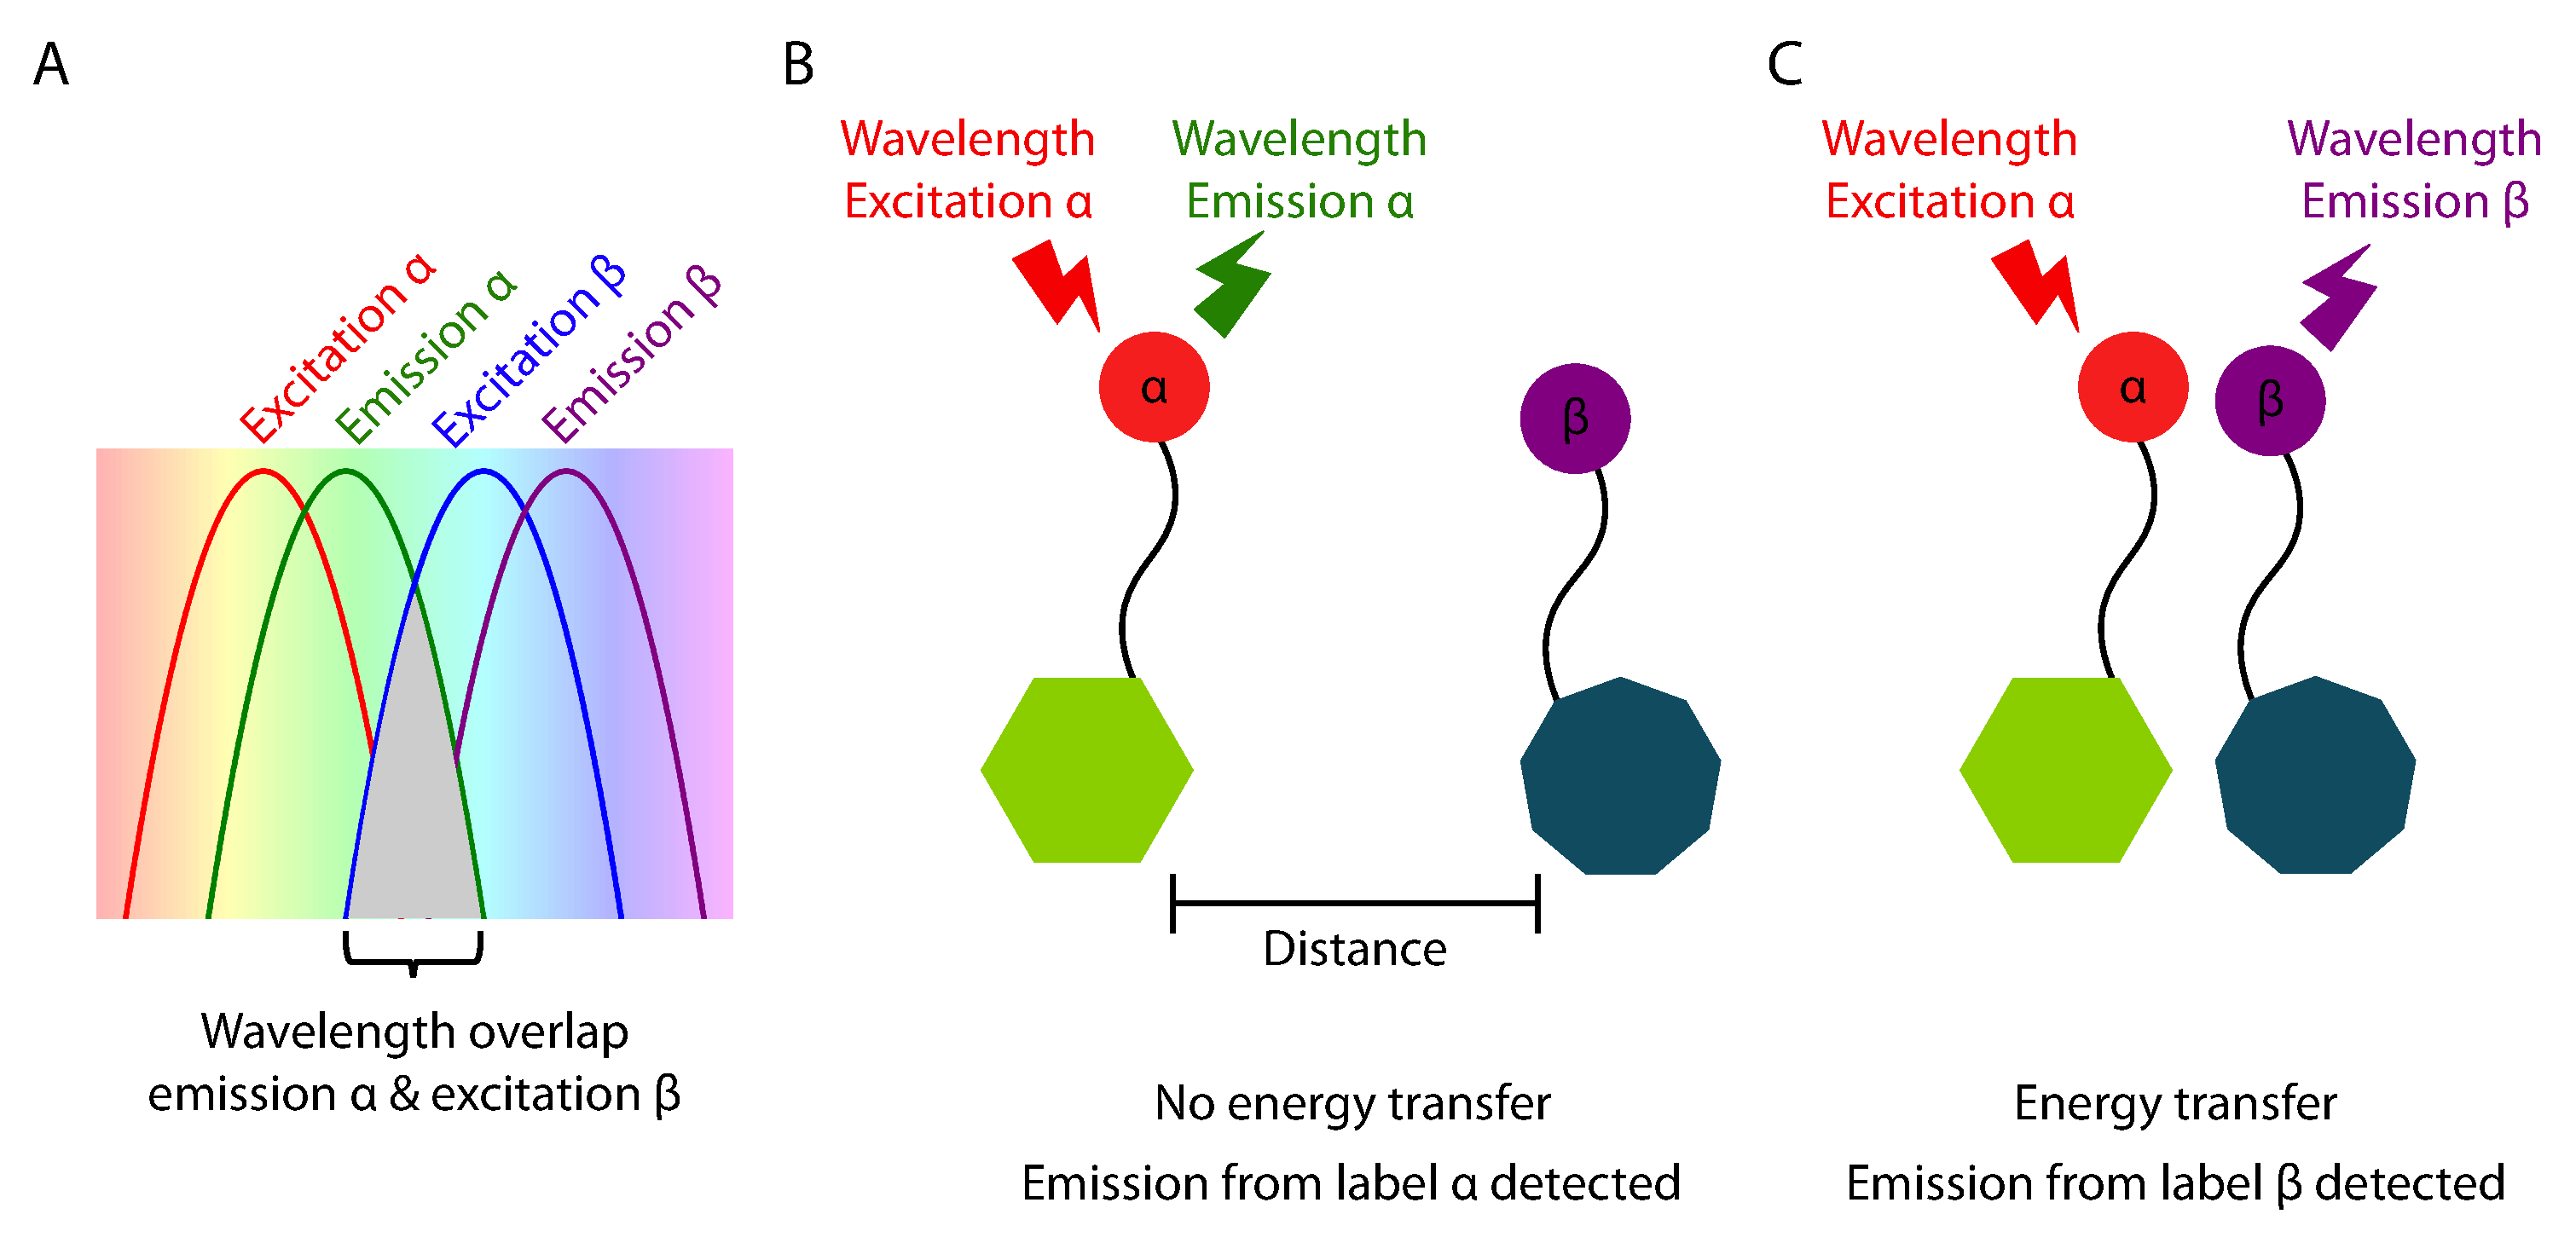
\includegraphics[width=1\linewidth]{figures/experimental_techniques_fret.pdf}
    \caption{\textbf{Förster Resonance Energy Transfer (FRET) mechanism.} A) The excitation and emission wavelengths of fluorescent dyes $\alpha$ and $\beta$. FRET is based on the energy transfer between two fluorescent dyes, in this example possible because dye $\alpha$'s emission wavelengths overlap with dye $\beta$ excitation wavelengths. B) Two distant proteins labelled with dyes $\alpha$ and $\beta$ and exposed to light with wavelength in the $\alpha$ excitation range. Energy cannot be transferred to dye $\beta$ and therefore dye $\alpha$ emits light. C) Two nearby proteins labelled with dyes $\alpha$ and $\beta$ and exposed to light with wavelength in the $\alpha$ excitation range. Energy is transferred from dyes $\alpha$ to $\beta$ and therefore dye $\beta$ emits light.}
    \label{fig:chapter1:fret}
\end{figure}

Other methods, such as Atomic Force \Gls{microscopy} (AFM), can be used not only to visualise molecules but also to study the folding and unfolding of proteins \cite{van_gils_protein_2024}. In addition to AFM's application in imaging, it can be used to pull from different regions of a protein and measure pulling forces, an application known as Single Molecule Force Spectroscopy (SMFS) \cite{hughes_physics_2016}. By attaching two protein regions to the AFM base and to the tip of its cantilever, the amino-acid chain can be pulled and relaxed to study its folding mechanics and \gls{dynamics} (\figref{fig:chapter1:afm}). Other techniques employ the same principle as AFM, but with different pulling strategies, namely Optical Tweezers \cite{bustamante_single-molecule_2020}, which pull with laser beams, or Magnetic Tweezers \cite{tapia-rojo_ephemeral_2019}, which pull with electro-magnetism.

\begin{figure}[tbh!]
    \centering
    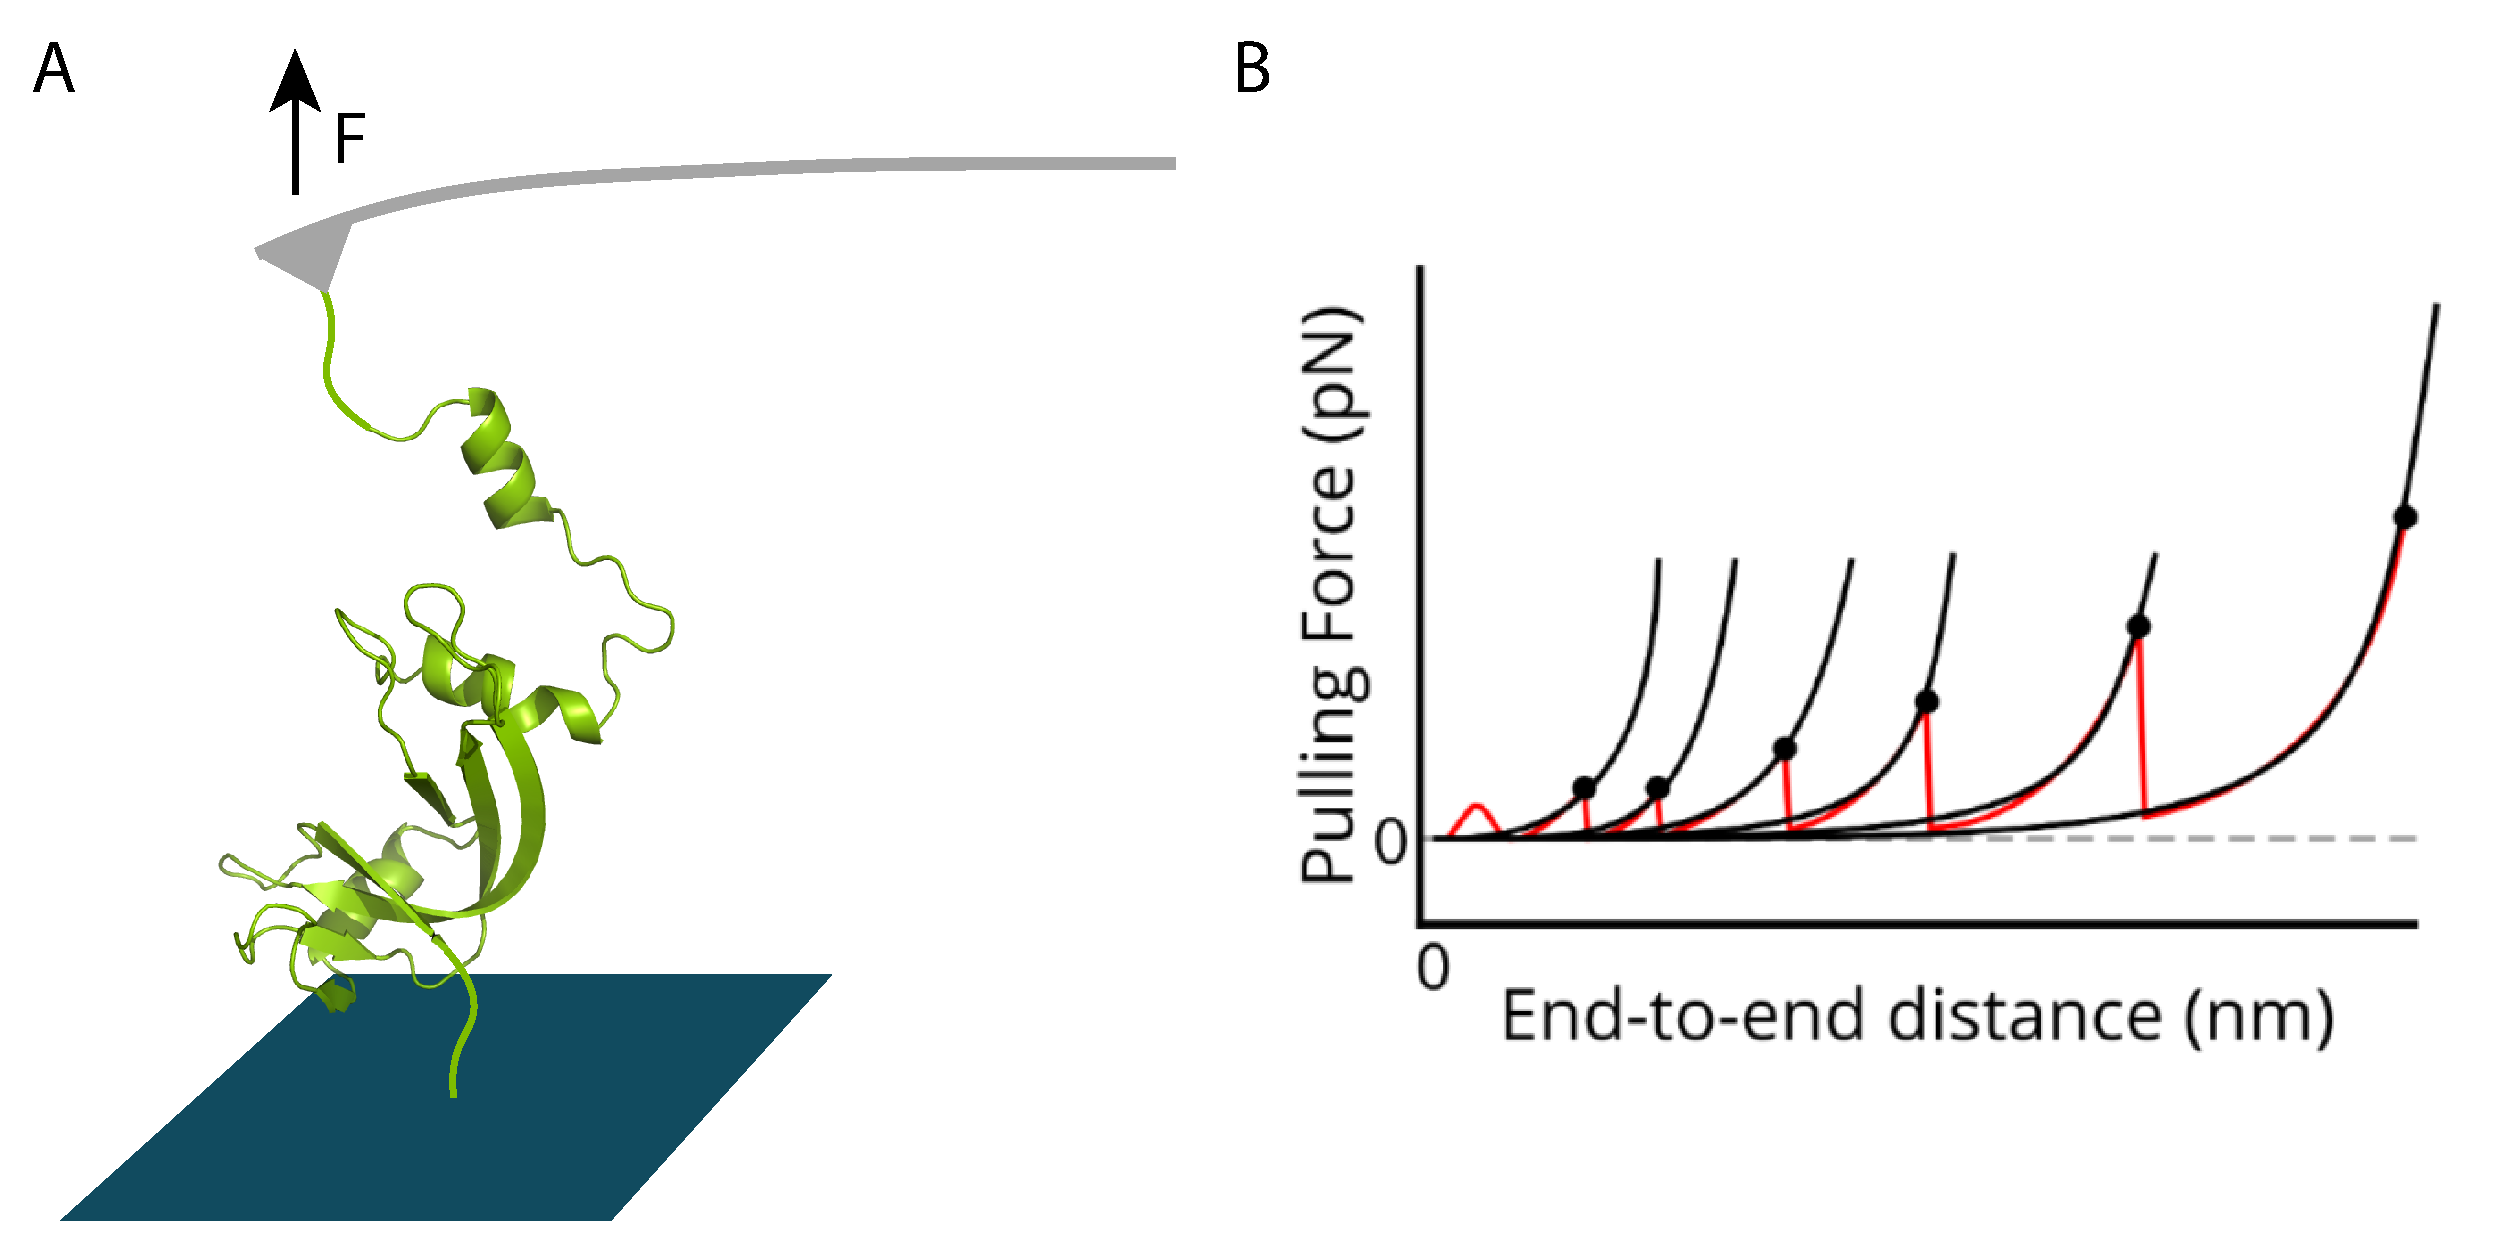
\includegraphics[width=1\linewidth]{figures/experimental_techniques_afm.pdf}
    \caption{\textbf{Atomic Force \Gls{microscopy} (AFM) pull-off force measurement.} A) A protein is attached to a base from one of its extremes and to the AFM cantilever from the other. The cantilever then pulls from the protein, gradually forcing it into a stretched \gls{conformation}. Pulling results on the sequential unfolding of the protein, which can be quantified by changes in pulling forces (PDB ID: 11BG \cite{vitagliano_potential_1999}). B) Force required to pull a protein to different extensions. Each peak indicates the loss of \gls{conformation} of a region (\textit{e.g.} a $\beta$-strand detached from a \gls{betasheet}). Subplot B extracted from \cite{van_gils_protein_2024}.}
    \label{fig:chapter1:afm}
\end{figure}


As much as these methods have been employed to elucidate the mechanisms and \gls{dynamics} of proteins, they rely either on labelling or on the binding of other external elements, which might interfere with the expected \textit{in vivo} \gls{dynamics}. 
Importantly, all the techniques discussed in this section are capable of measuring the behaviour of individual proteins, which might not be immediately obvious for some methods. For instance, whilst it is clear that AFM pull assays can monitor single molecules by stretching a single protein, other techniques (\textit{e.g.} FRET) can also be adapted to single-molecule studies. These techniques enable
the study of \gls{dynamics} across relatively large regions of a protein rather than at the per-residue level, which is central for understanding protein collective motions and conformational changes.


\subsection{Residue-Level Indirect Dynamic Measurements}

Several methods suited for protein structural determination have proven to be useful in the study of protein \gls{dynamics}. Here I will focus on \gls{xraycrystallography} crystallography and cryogenic electron \gls{microscopy} (\gls{cryoem}), both nowadays capable of producing structural models of proteins up to the atomic resolution \cite{yip_atomic-resolution_2020}. Although both \gls{xraycrystallography} and \gls{cryoem} can be used to model a single protein structure, their direct measurements reflect the conformations of multiple protein molecules rather than a single molecule. These techniques produce the vast majority of all available experimental \glspl{proteinstructure} \cite{noauthor_pdb_nodate_overal_statistics, noauthor_pdb_nodate_xray, noauthor_pdb_nodate_nmr, noauthor_pdb_nodate_cryoem}, which is also their most common application. These techniques occur under cryogenic and dehydrated conditions, far from \gls{physiologicalconditions}, to reduce protein motions as much as possible and thus increase resolution. Even under such non-native experimental conditions, there are strategies to study the dynamic properties of a protein from these structures. For instance, the conformational diversity of a protein with multiple defined \glspl{conformation} can be approximated simply by structurally aligning multiple static structures of the same protein \cite{monzon_codnas_2013, monzon_codnas_2016}. 


\gls{xraycrystallography} crystallography is a technique employed to obtain static \glspl{proteinstructure}. The sample preparation for this technique requires the crystallisation of the studied proteins. This process is non-trivial and often requires very dynamic protein regions to be trimmed to form the crystal or to prevent it from cracking due to large \gls{proteindomain} movements \cite{mooij_proteinccd_2009, gavrilov_nmr_2018}. Once the crystal is formed, an \gls{xraycrystallography} beam is passed through it, which will be diffracted by the protein's \glspl{electron}. The deflection pattern, which depends on the location of a protein's \glspl{electron}, is captured and modelled into a \gls{proteinstructure}. On individual \gls{xraycrystallography} structures, the low resolution or inability to model certain residues indicates that their atom's \gls{electron} cloud was too spread for assigning spatial coordinates \cite{smyth_x_2000}, thereby indicating considerable motion. For modelled residues, high \gls{electron} spread, hence low positional certainty and higher \gls{flexibility}, is represented with high residue \glspl{bfactor}---a metric of \gls{electron} density distribution in crystallography \cite{smyth_x_2000, carugo_b-factor_2022}; conversely, low \glspl{bfactor} indicate reduced \gls{electron} dispersion, higher positional certainty, and less \gls{flexibility}.


\Gls{cryoem} is a technique that does not require crystallisation, but it requires the protein samples to be rapidly cooled to reduce molecular motion and keep proteins near their native \gls{conformation} in a process named vitrification \cite{naydenova_reduction_2022, pfeil-gardiner_comparative_2019, bock_effects_2022, engstrom_high-resolution_2021}. These samples are then photographed in 2-dimensions with electron \gls{microscopy} (\glspl{electronmicroscopy}) from different angles, which will be computationally reconstructed into a 3-dimensional model of the protein. \Gls{cryoem} features equivalent metrics to \gls{xraycrystallography}'s \glspl{bfactor}, such as an \gls{aminoacid}'s local resolution \cite{yip_atomic-resolution_2020}, which also relates to the spread of a residue's \gls{electron} density. The interpretation of both these metrics carries an important consideration: though these metrics are based on quantifiable physical principles like \gls{electron} density and spread, they are still measured under conditions far from those in which the protein can be found \textit{in vivo} and therefore only proxy protein \gls{dynamics} under these non-\gls{physiologicalconditions}. It is not correct to extrapolate these measurements to \gls{physiologicalconditions}.

\subsection{Nuclear Magnetic Resonance Spectroscopy for Direct Dynamic Measurement}

A more adequate approach to studying protein \gls{dynamics} under near-\gls{physiologicalconditions} is the use of Nuclear Magnetic Resonance spectroscopy (\gls{nmr}), which allows in-solution measurements at physiological temperatures \cite{kleckner_introduction_2011, kuloglu_structural_2002}. \gls{nmr} applied to structure determination generates an ensemble of modelled structures, which serves as a sampling of a protein's conformationally allowed space.

Briefly, \gls{nmr} can identify the environment of an atom of interest with a 1/2 \gls{nuclearspin} \gls{nucleus} (atoms with specific configurations of \glspl{proton} and \glspl{neutron}), which makes the atom have a non-zero nuclear \gls{nuclearspin} (\figref{fig:chapter1:atom}). This confers the atoms magnetic properties, which can interact with a \gls{magneticfield} (\textit{e.g.} $^{1}\text{H}$ or simply ``\gls{proton}'', or $^{13}\text{C}$). These atoms are analysed based on the following basic principle: First, a strong \gls{magneticfield} is applied to a protein (or any other molecule), thereby aligning the \gls{nuclearspin} of its \gls{nucleus} with the direction of the \gls{magneticfield} \cite{marion_introduction_2013}. Then, an orthogonal \glspl{radiofrequency} (\gls{radiofrequency}) is pulsed, which temporarily shifts the orientation of the \glspl{nucleus}'s \gls{nuclearspin}. The \gls{electron} cloud of each atom and its neighbouring atoms determines the local magnetic environment and thus offers the \gls{nucleus} a different degree of shielding \cite{marion_introduction_2013}, which results in larger or smaller \gls{nuclearspin} transition and hence larger or smaller \glspl{chemicalshift}. As the \gls{nucleus}' \gls{nuclearspin} re-aligns with the original \gls{magneticfield}, changes in the \gls{magneticfield} at specific frequencies are detected by a coil surrounding the sample. These changes induce an electrical signal in the coil, which provides information about the \gls{nucleus}' degree of shielding when the \gls{radiofrequency} was applied. These frequencies are measured at once for all atoms of interest for each molecule in the sample, and then Fourier-transformed into spectra. The peaks in the spectra are then compared with the frequency of a reference standard, and measured in \glspl{ppm} (ppm). 
Given the size, connectivity and complexity of proteins, additional experiments are needed to resolve their structures, leading to the development of multi-dimensional \gls{nmr} methods. Some of these methods include \gls{cosy} (Correlated Spectroscopy), \gls{noesy} (Nuclear Overhauser Effect Spectroscopy) and \gls{hsqc} (Heteronuclear Single Quantum Coherence)  \cite{kline_determination_1988, kwan_macromolecular_2011}.

% \textcolor{red}{The NMR structural ensembles offer a range of conformations in which the protein can exist rather than structures of single molecules. In other words, every single model in the structural ensemble is derived from a population of molecules rather than capturing individual behaviours. In order to interpret the conformational space of a protein, ensemble averaging [ref], can be applied. This technique averages the coordinates of selected atoms (often those forming the protein backbone) to obtain an averaged or consensus structure. The spread of atomic coordinates can be calculated to obtain a measure of flexibility. This method allows a purely coordinate-based numerical representation of protein conformation and flexibility from NMR ensembles.}

\textcolor{red}{The NMR structural ensembles represent a range of conformations in which the protein can exist, reflecting the diverse structural states sampled by a population of molecules rather than individual static structures. Each model within the ensemble thus captures the collective behaviour of the molecular population, encompassing multiple conformations. Since NMR data yield an ensemble-averaged view of structural parameters---such as bond distances, angles, and dihedral angles---this averaging represents a comprehensive depiction of the protein’s conformational landscape rather than any single static structure. By averaging all these parameters across the entire ensemble, NMR provides insights into regions of stability and flexibility, as the ensemble reflects both the most probable structural features and the extent of their variation. In this way, ensemble-averaged parameters enable a probabilistic understanding of the protein’s structural landscape, suggesting areas of rigidity where parameter variation is low and regions of flexibility where it is high \cite{sutcliffe_representing_1993, stockelmaier_conformational_2024}. Although the ensemble does not capture dynamic transitions or timescales, it provides a statistical summary of the conformational possibilities that indicate the likely dynamic properties of the protein.}

% By analysing these conformational averages, we gain a deeper understanding of the protein’s potential functional motions, as each conformation represents not only a possible structure but also the likelihood of transitions between states, offering a window into the dynamic properties that may underpin its biological function.}

% \textcolor{red}{The NMR structural ensembles represent a range of conformations in which the protein can exist, reflecting the diverse structural states sampled by a population of molecules rather than individual static structures. Each model within the ensemble thus captures the collective behaviour of the molecular population, encompassing multiple conformations. As the data obtained from NMR represent averages, an interpretation of these ensembles is their own average...

% Ensemble averaging can be applied to obtain a representative conformation of 

% interpret this conformational space quantitatively, ensemble averaging \cite{sutcliffe_representing_1993} can be applied. }

% This technique involves averaging the coordinates of selected atoms, often those in the protein backbone, to derive an averaged or consensus structure. Additionally, calculating the spread of atomic coordinates provides a measure of flexibility for each region. Through this approach, ensemble averaging allows a coordinate-based, numerical representation of protein conformation and flexibility, directly derived from NMR ensembles.}


\begin{figure}[tbh!]
    \centering
    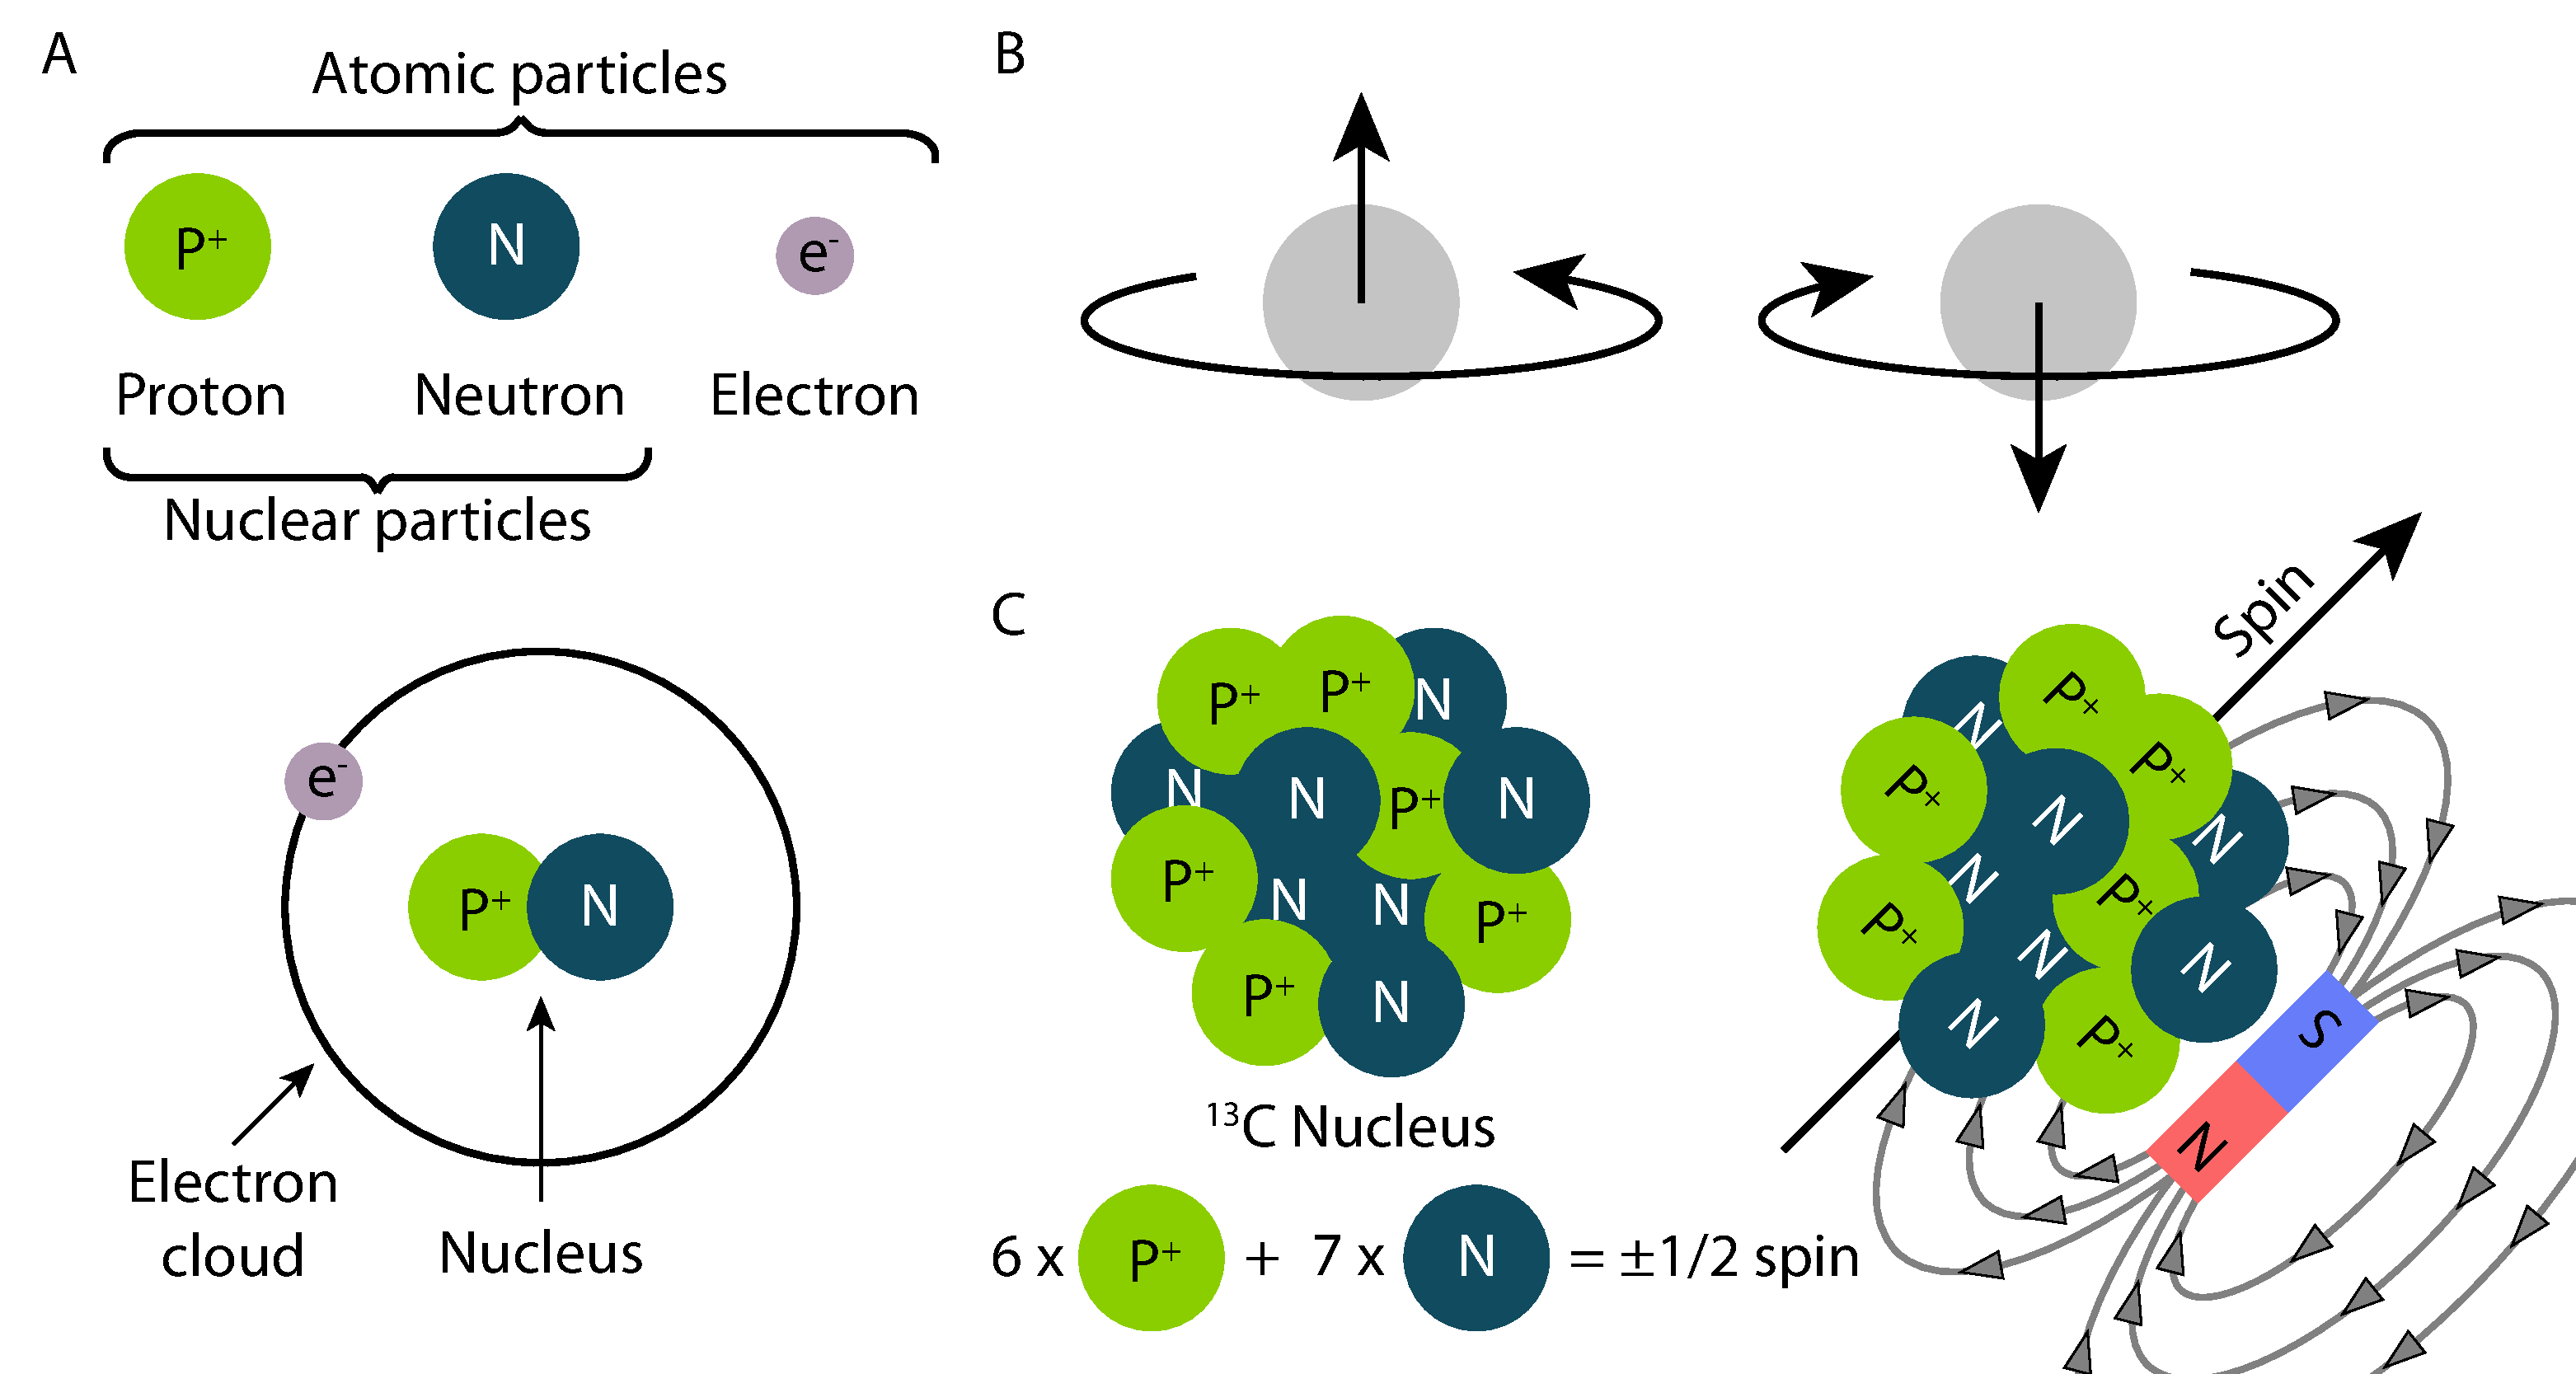
\includegraphics[width=1\linewidth]{figures/spin_nucleous.pdf}
    \caption{\textbf{Atom components and nuclear \gls{nuclearspin}.} A) An atom is composed of a combination of \glspl{proton}, \glspl{neutron} and \glspl{electron}, named atomic particles. \Glspl{proton} and \glspl{neutron} are located in the \gls{nucleus} of an atom and thereby constituting a subset of atomic particles: the nuclear particles. The \glspl{electron} exist in a cloud surrounding the \gls{nucleus}. B) Each atomic particle has an intrinsic angular momentum or \gls{nuclearspin}, which can be, in the case of atomic particles, projected as either ``up'' or ``down'' (different spins are allowed for other particles, but atomic particles feature only these two). This angular momentum is also called \gls{nuclearspin} because the behaviour of the particle is analogous to a sphere rotating with either right-hand or left-hand spinning, although the particles do not actually physically \gls{nuclearspin}. Atomic particles, specifically \glspl{proton}, \glspl{neutron}, and \glspl{electron}, are fermions (particles with half-integer \gls{nuclearspin}) with a \gls{nuclearspin} of 1/2. The allowed \gls{nuclearspin} projections for these particles are +1/2 and -1/2. C) The \gls{nucleus} of $^{13}\text{C}$ contains 6 \glspl{proton} and 7 \glspl{neutron}, which cannot balance each other out and therefore, the total nuclear \gls{nuclearspin} is ±1/2. This confers magnetic properties to the \gls{nucleus}, which can thereby be induced into an orientation by a \gls{magneticfield}. In this example, the \gls{nucleus} has a +1/2 \gls{nuclearspin} projection, and is thereby oriented in the same direction as the \gls{magneticfield}. 
    }
    \label{fig:chapter1:atom}
\end{figure}

\begin{figure}[tbh!]
    \centering
    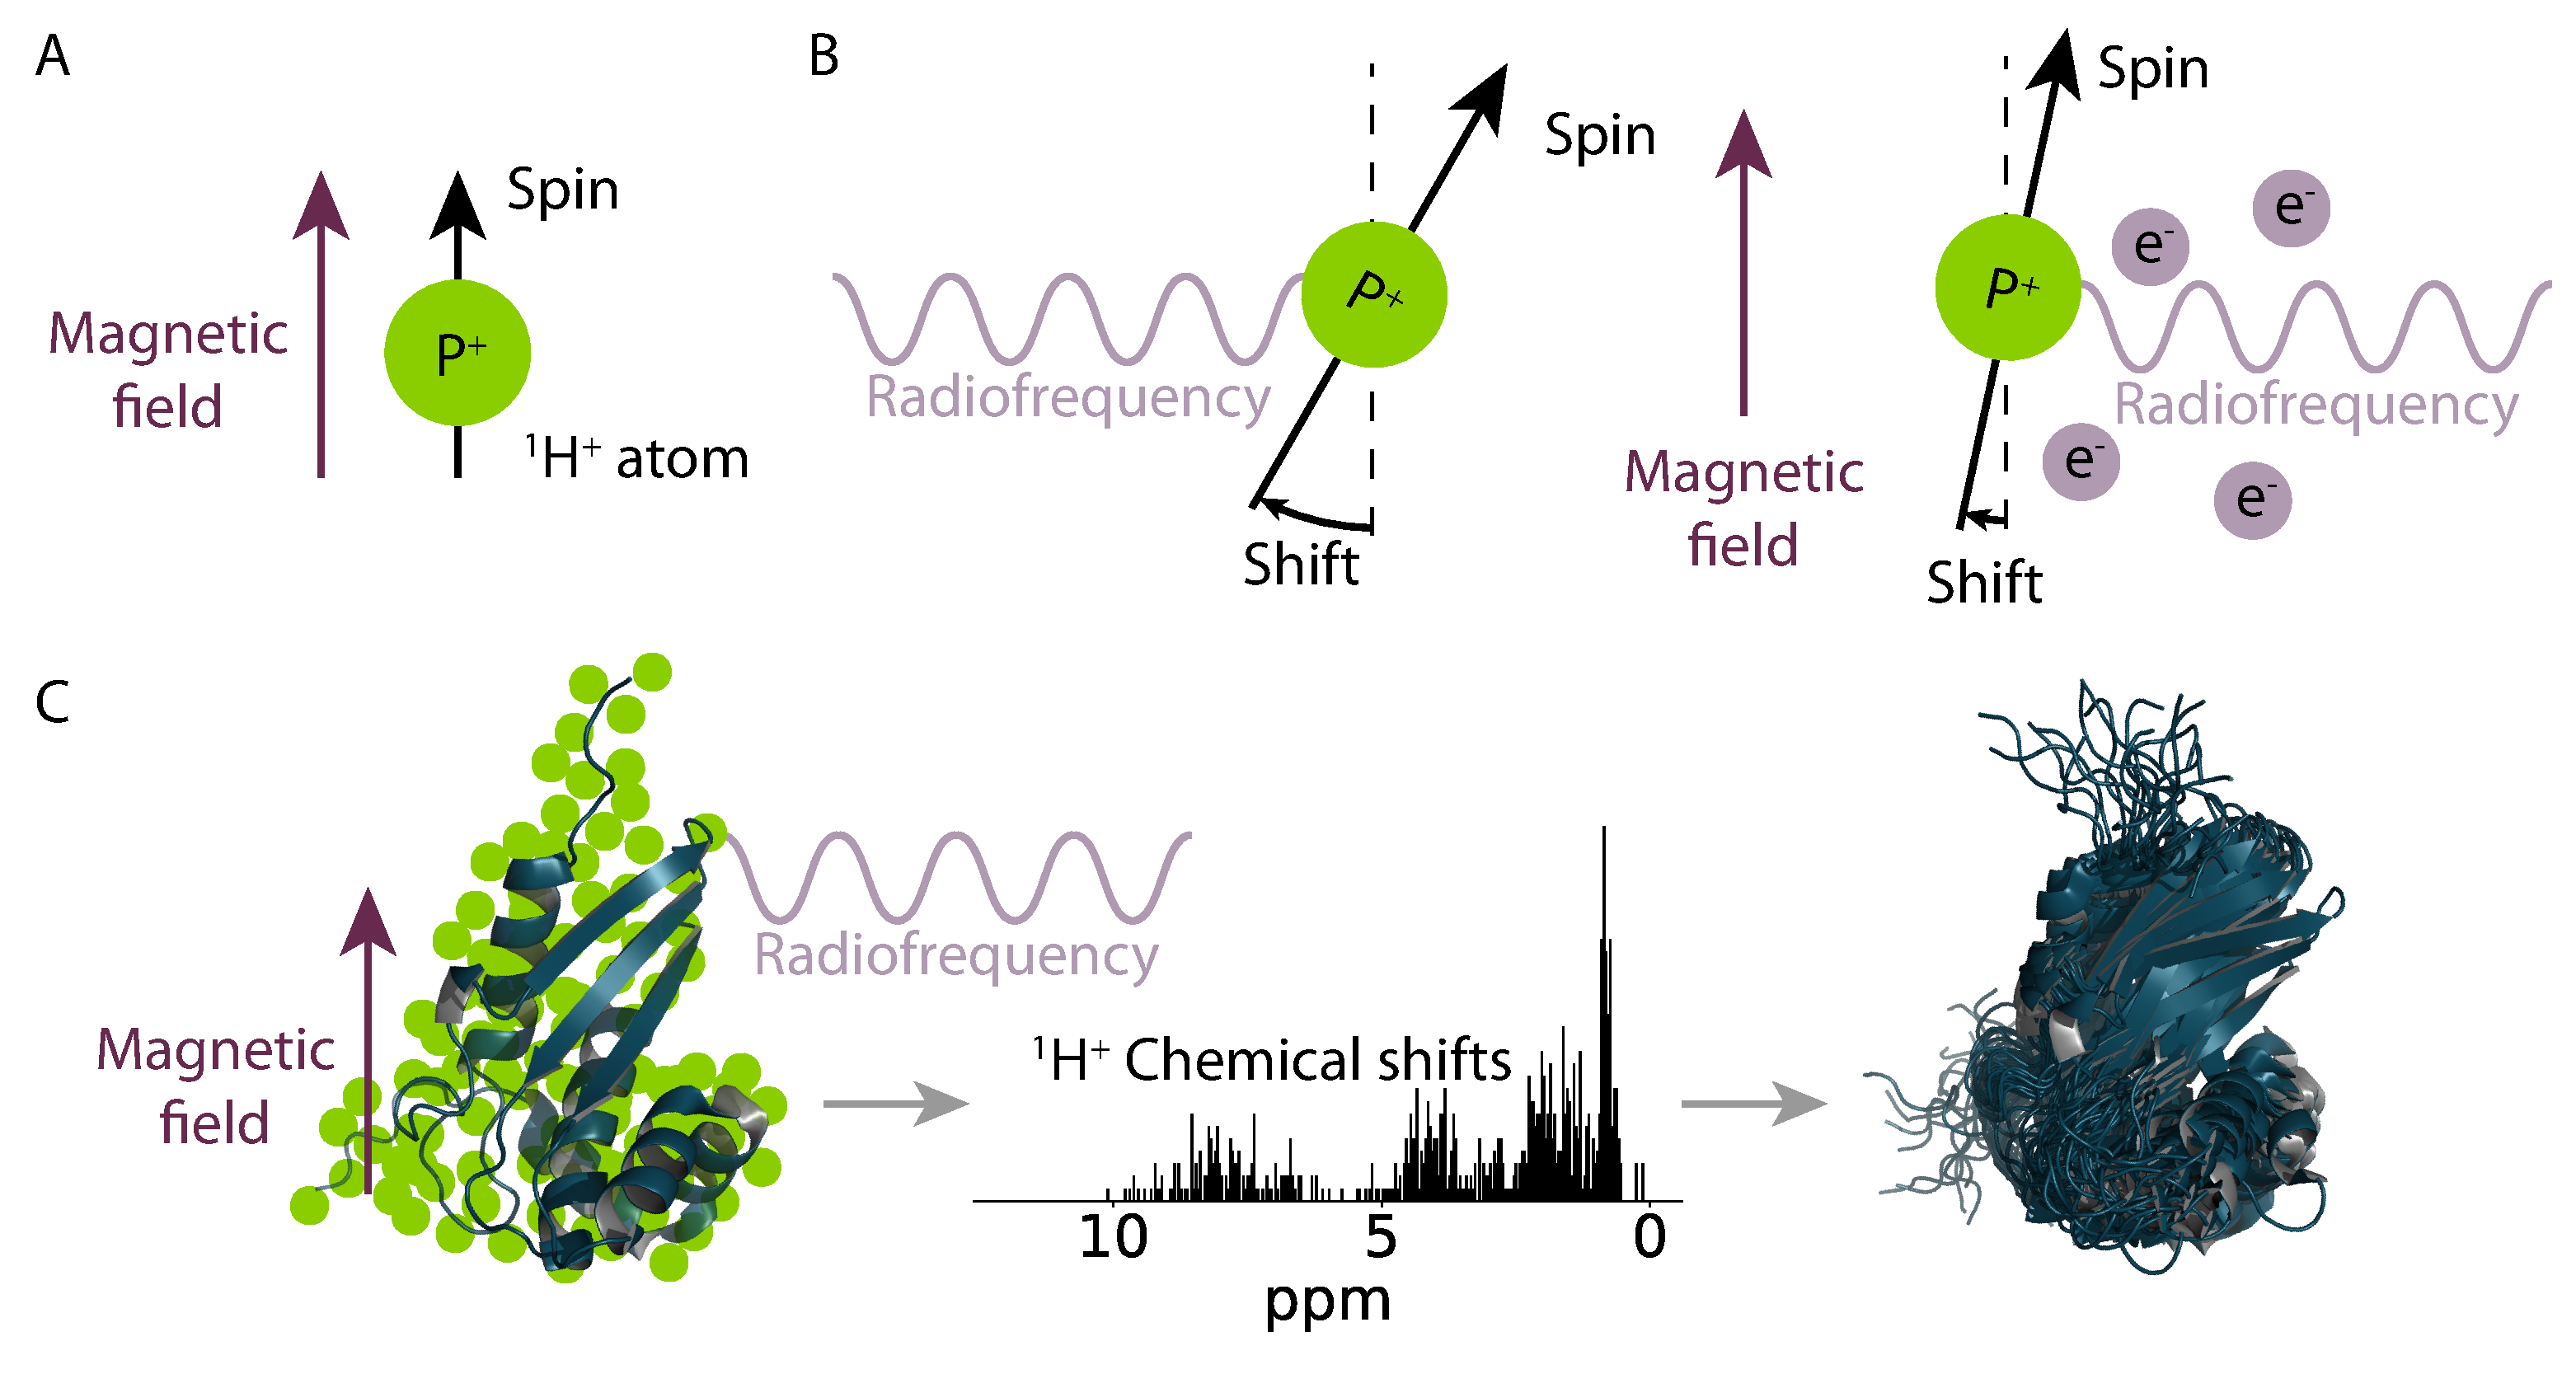
\includegraphics[width=1\linewidth]{figures/nmr_guts.pdf}
    \caption{\textbf{\gls{nmr} fundamentals illustrated with \gls{proton} \gls{nmr}.} A) The \gls{proton} in this example has a +1/2 \gls{nuclearspin} projection, therefore aligning to the \gls{magneticfield} generated by the \gls{nmr} machine (machine omitted in figure). B) The \gls{proton} is disturbed by a radiofrequency (\gls{radiofrequency}), perpendicular to the \gls{magneticfield}, which shifts the orientation of the \gls{proton}'s \gls{nuclearspin}. The \gls{proton} can be shielded in different degrees from the \gls{radiofrequency}, resulting in smaller shifts than an unshielded \gls{proton}. C) At the protein level, there are multitude of \gls{proton} atoms, each with different degree of \gls{electron} shielding, depending on their molecular context (their location in the protein). When the protein is perturbed with a \gls{radiofrequency}, \glspl{proton} shift their \gls{nuclearspin} alignment from the \gls{magneticfield}. While the \glspl{nucleus} \gls{nuclearspin} re-align with the \gls{magneticfield}, they induce electrical signals in the \gls{nmr} machine's detection coil, which captures their frequencies. These frequencies can be used to model the \gls{proteinstructure} as an ensemble of models, each representing an allowed \gls{conformation} for such protein. The \glspl{proteinstructure} in this figure  are models in the ensemble PDB ID 2M5H \cite{ouyang_solution_2013}.}
    \label{fig:chapter1:nmr}
\end{figure}


Beyond structure determination, \gls{nmr} can also be applied to the study of protein motions at the residue level. Two \gls{nmr} metrics are prominent in the study of protein motions: Random Coil Index (\gls{rci}) and $\text{S}^{2}$ order parameter (\gls{s2orderparameter}). \gls{rci} is a metric derived from comparing the \gls{chemicalshift} of an \gls{aminoacid}'s \glspl{nucleus} versus the expected unstructured \gls{chemicalshift} of such \gls{aminoacid} \cite{schwarzinger_random_2000}. This metric, therefore, offers a description of an \gls{aminoacid}'s \gls{flexibility} at slow time scales (micro- to milli-seconds), where near-zero values represent unstructured regions which can easily change \gls{conformation}, such as coil or turn, and higher values represent structured, more rigid \glspl{conformation}, such as \gls{alphahelix} or \gls{betasheet}. \gls{s2orderparameter}, on the other hand, offers a direct measurement of protein \gls{dynamics} at short time scales (pico- to nano-seconds) \cite{sapienza_using_2010}. It does so by measuring the amplitude of motion of the N-H (for \gls{backbone} dynamics) or C-H (for \gls{sidechain} dynamics) vectors relative to the protein \gls{backbone} after \gls{radiofrequency} perturbation \cite{sapienza_using_2010, smith_use_2021}. Together, they offer an overview of protein \gls{dynamics} and conformational tendencies at different time scales.


Some other variants of \gls{nmr} facilitate the study of diverse aspects of protein \gls{dynamics}, folding, and binding \cite{kleckner_introduction_2011}. Examples of these variants are real-time (RT) \gls{nmr} and residual dipolar coupling (RDC). 
RT-\gls{nmr} provides information about the structural evolution of proteins subject to a certain environment. It does so by measuring \gls{nmr} spectra over time after the introduction of a new condition (\textit{e.g.} the addition of a binder). Over time, the intensity from the frequencies in the starting \glspl{conformation} diminish as the ones from the final \glspl{conformation} increase \cite{zeeb_protein_2004}. 
RDC arises when molecules experience partial alignment in a \gls{magneticfield}, leading to detectable dipolar interactions between nuclear spins. RDCs offer angular constraints that reveal relative orientations and distances of protein domains, providing insights into the global fold and conformational changes of proteins \cite{tolman_nmr_2006}. This technique requires special alignment media to induce partial alignment, unlike RT-\gls{nmr}, which can be measured under standard \gls{nmr} conditions. RDCs are particularly useful for studying large proteins and complexes, complementing traditional \gls{nmr} techniques by providing long-range structural information \cite{tolman_novel_2002, bax_weak_2003}.

This brief introduction to \gls{nmr} focuses on protein structural diversity, \gls{flexibility}, and \gls{dynamics}, but this technique's polyvalence enables applications such as the study of folding mechanisms \cite{peacock_hydrogendeuterium_2021}, the observation of conformational changes at different temperature and pH ranges \cite{gerken_measurement_2011}, and binding mechanics \cite{dubey_role_2020}. Notable drawbacks of \gls{nmr} are the difficulties in studying large proteins \cite{frueh_nmr_2013} and the lower resolution of its elucidated structures compared to \gls{xraycrystallography} crystallography or \gls{cryoem} \cite{kwan_macromolecular_2011}. Arguably, the latter is not a drawback, but a feature created by the motion of proteins in near-\gls{physiologicalconditions}.

\subsection{\textcolor{red}{Complementary Spectroscopic Techniques}}

\textcolor{red}{In addition to NMR, other spectroscopic techniques, such as Electron Paramagnetic Resonance (EPR) and Circular Dichroism (CD), provide complementary insights into protein dynamics at the molecular level. EPR spectroscopy is used to investigate molecular interactions by measuring the magnetic properties of unpaired electrons (\textit{e.i.} electrons that solely occupy an orbital) introduced through site-specific spin labelling. This method enables precise measurement of distances in the nm range, making it suitable for detecting conformational changes and the motion of labelled sites within proteins \cite{sahu_electron_2020}.}

\textcolor{red}{CD spectroscopy, on the other hand, assesses secondary structural content by examining the differential absorption of left- and right-handed circularly polarised light. These two polarisation types interact differently with chiral molecules, like proteins, and are absorbed to varying degrees depending on the secondary structure. $\alpha$-helices, $\beta$-sheets, and random coils each have distinct CD spectra, as the unique chiral arrangements within these structures selectively absorb and rotate polarised light to differing extents \cite{greenfield_using_2006}. Changes protein conformation are directly related to variations in CD spectra. By capturing these variations, CD enables analysis of protein folding, stability, and structural transitions under various conditions.}

\section{Computational Study of Protein Motions}
\subsection{Molecular Dynamics}

Beyond the insights on protein conformational diversity and protein \gls{dynamics} that experimental methods can provide, diverse computational methods offer complementary information on a protein's dynamic nature. Notably, the use of Molecular Dynamics (\gls{md}) simulations is a flexible method that can be applied to problems such as drug-target binding \cite{de_vivo_role_2016}, effects of post-translational modifications \cite{sostaric_molecular_2021, bickel_effects_2024}, and the study of \glspl{idp} \cite{shrestha_full_2021}. 
In \gls{md} simulations, molecules are represented by a Newtonian physics model, where interactions are depicted as mechanical forces, such as Hooke's law \cite{adcock_molecular_2006}. Numerical integration over these forces allows the simulation of molecular motion over time, which generates time series of \glspl{conformation} or structures known as trajectories \cite{adcock_molecular_2006}.
\gls{md} simulations calculate the trajectories that a molecular system (\textit{e.g.} a protein monomer in solution) follows over a period of time (typically nano- to milli-seconds) \cite{lindorff-larsen_picosecond_2016}. 

These trajectories are calculated by first setting up the molecular system with initial coordinates and velocities, where velocities are the speeds and directions of atomic movement. The system's interactions are defined using a force field, a mathematical model that describes the potential energy of the system as a function of atomic positions. This includes terms for bonded interactions (bonds, angles, dihedrals) and non-bonded interactions (\gls{vandewaalsforces}, \gls{electrostaticinteractions}). After energy minimisation to remove steric clashes (unrealistically close contacts between atoms that cause high repulsive forces), the system is equilibrated to the desired temperature and pressure. Newton's equations of motion are then solved iteratively using numerical integration methods which consider atomic position, velocity, and acceleration (like the Verlet algorithm) to update atomic positions and velocities over time. These coordinates are saved at regular intervals, creating a time series of molecular \glspl{conformation} called trajectories. The sequential nature of these trajectories, the sampled structures in the \gls{md} simulation can be analysed as a timeline, possibly elucidating mechanisms that would be observed with difficulty from \gls{nmr} ensembles. 

Some metrics to extract information from \gls{md} simulations include Root Mean Square Deviation (\gls{rmsd}), Root Mean Square Fluctuations (\gls{rmsf}), and Circular Variance (\gls{cv}), which measure a protein's \gls{flexibility} both in the \gls{cartesianspace} or \gls{dihedralspace}. The \gls{rmsd} is a global metric of coordinate deviation from a reference structure, which can be used to simply identify large conformational changes through the trajectory. The \gls{rmsf} is a local per-residue (or atom) measure of deviation from a reference structure. Similarly to \gls{rmsd}, it can be used to detect changes in \glspl{conformation}, but it also identifies which residues are more affected by such changes. Both \gls{rmsd} and \gls{rmsf} are dependent on structural superposition to a reference structure, and thus sensitive to large structural shifts with a distant origin, such as those stemming from hinge regions. The \gls{cv} measures the changes in a residue's $\phi$ and $\psi$ angles over the course of an \gls{md} simulation. This makes the method superposition-independent, especially useful for proteins where a canonical reference structure is not available, such as IDPs or \glspl{idr}. Following the previous example, distant residues from the hinge region will not be deemed as highly motile, as with \gls{rmsf}, unless they experience dihedral changes themselves. In the context of this thesis, \gls{md} simulations were used to generate \gls{conformation} ensembles of a wide variety of proteins which were further analysed with Constava, a method developed as part of this work to quantify the allowed range of conformational states that proteins are capable of adopting and their capacity to transition among them (chapters \ref{chapter:contributions} and \ref{chapter:constava}).

\subsection{Normal Mode Analysis}

Another computational method to study protein motions is Normal Mode Analysis (\gls{nma}). This method calculates harmonic fluctuations around a \gls{proteinstructure}, in a computationally inexpensive manner, assuming that such structure represents the protein's \gls{globalminima} energy state \cite{wako_normal_2017}. While \gls{nma} can detect large-scale movements such as \gls{proteindomain} motions, it is limited by its harmonic and linear nature. \gls{md} simulations, on the other hand, are not restricted to linear motions and can more accurately describe complex conformational changes. Nevertheless, \gls{nma} is a powerful tool for rapidly probing a protein's \gls{flexibility} or to be applied to large-scale analysis due to its low computational requirements, as it was employed for the large-scale analysis of AlphaFold2 models in chapter \ref{chapter:plddt}.


\section{Protein Biophysics Computational Tools}

\subsection{Machine Learning in Biological Research}

Biological research has employed computational methods beyond the calculation of trajectories and harmonic movements. The development of data-centred models enables the quick extraction of information from a biological system, its analysis, and the definition of a set of labels or characteristics. These models perform their analysis in a structured manner, following a set of quantitative rules that determine the output of a system's analysis. This approach contrasts with human assessments, which are more prone to the introduction of qualitative criteria. The simplest family of models is the rule-based models, which are programmed to operate based on a predefined set of rules set by human experts (\textit{e.g.} a manually-created decision tree to determine from a \gls{proteinstructure} whether an \gls{aminoacid} is part of an \gls{alphahelix}). In contrast to this strategy are Machine Learning (\gls{machinelearning}) models, which learn the rules to perform a task from exposure to data. \gls{machinelearning} models require the definition of a model structure to be trained by exposing it to relevant data to learn how to perform a task (\figref{fig:chapter1:ml_basics}). \Glspl{supervisedlearning} \gls{machinelearning} models require the presence of labelled data for their training, which are employed for applications such as medical diagnosis \cite{kourou_machine_2015, capper_dna_2018}, personalised toxicity prediction \cite{vo_overview_2020, badwan_machine_2023}, and the estimation of protein properties \cite{cilia_protein_2013, orlando_accurate_2020, raimondi_exploring_2017, orlando_prediction_2022}. \Glspl{unsupervisedlearning} models are also widely used in biology to learn the structure of data \cite{chou_predicting_2006, maisuradze_principal_2009} or for feature extraction \cite{vaswani_attention_2023, church_word2vec_2017}. Complex model structures allow the combination of \gls{supervisedlearning} and \glspl{unsupervisedlearning} models. For the purpose of this work, we will focus on \glspl{supervisedlearning} models.


\begin{figure}[tbh!]
    \centering
    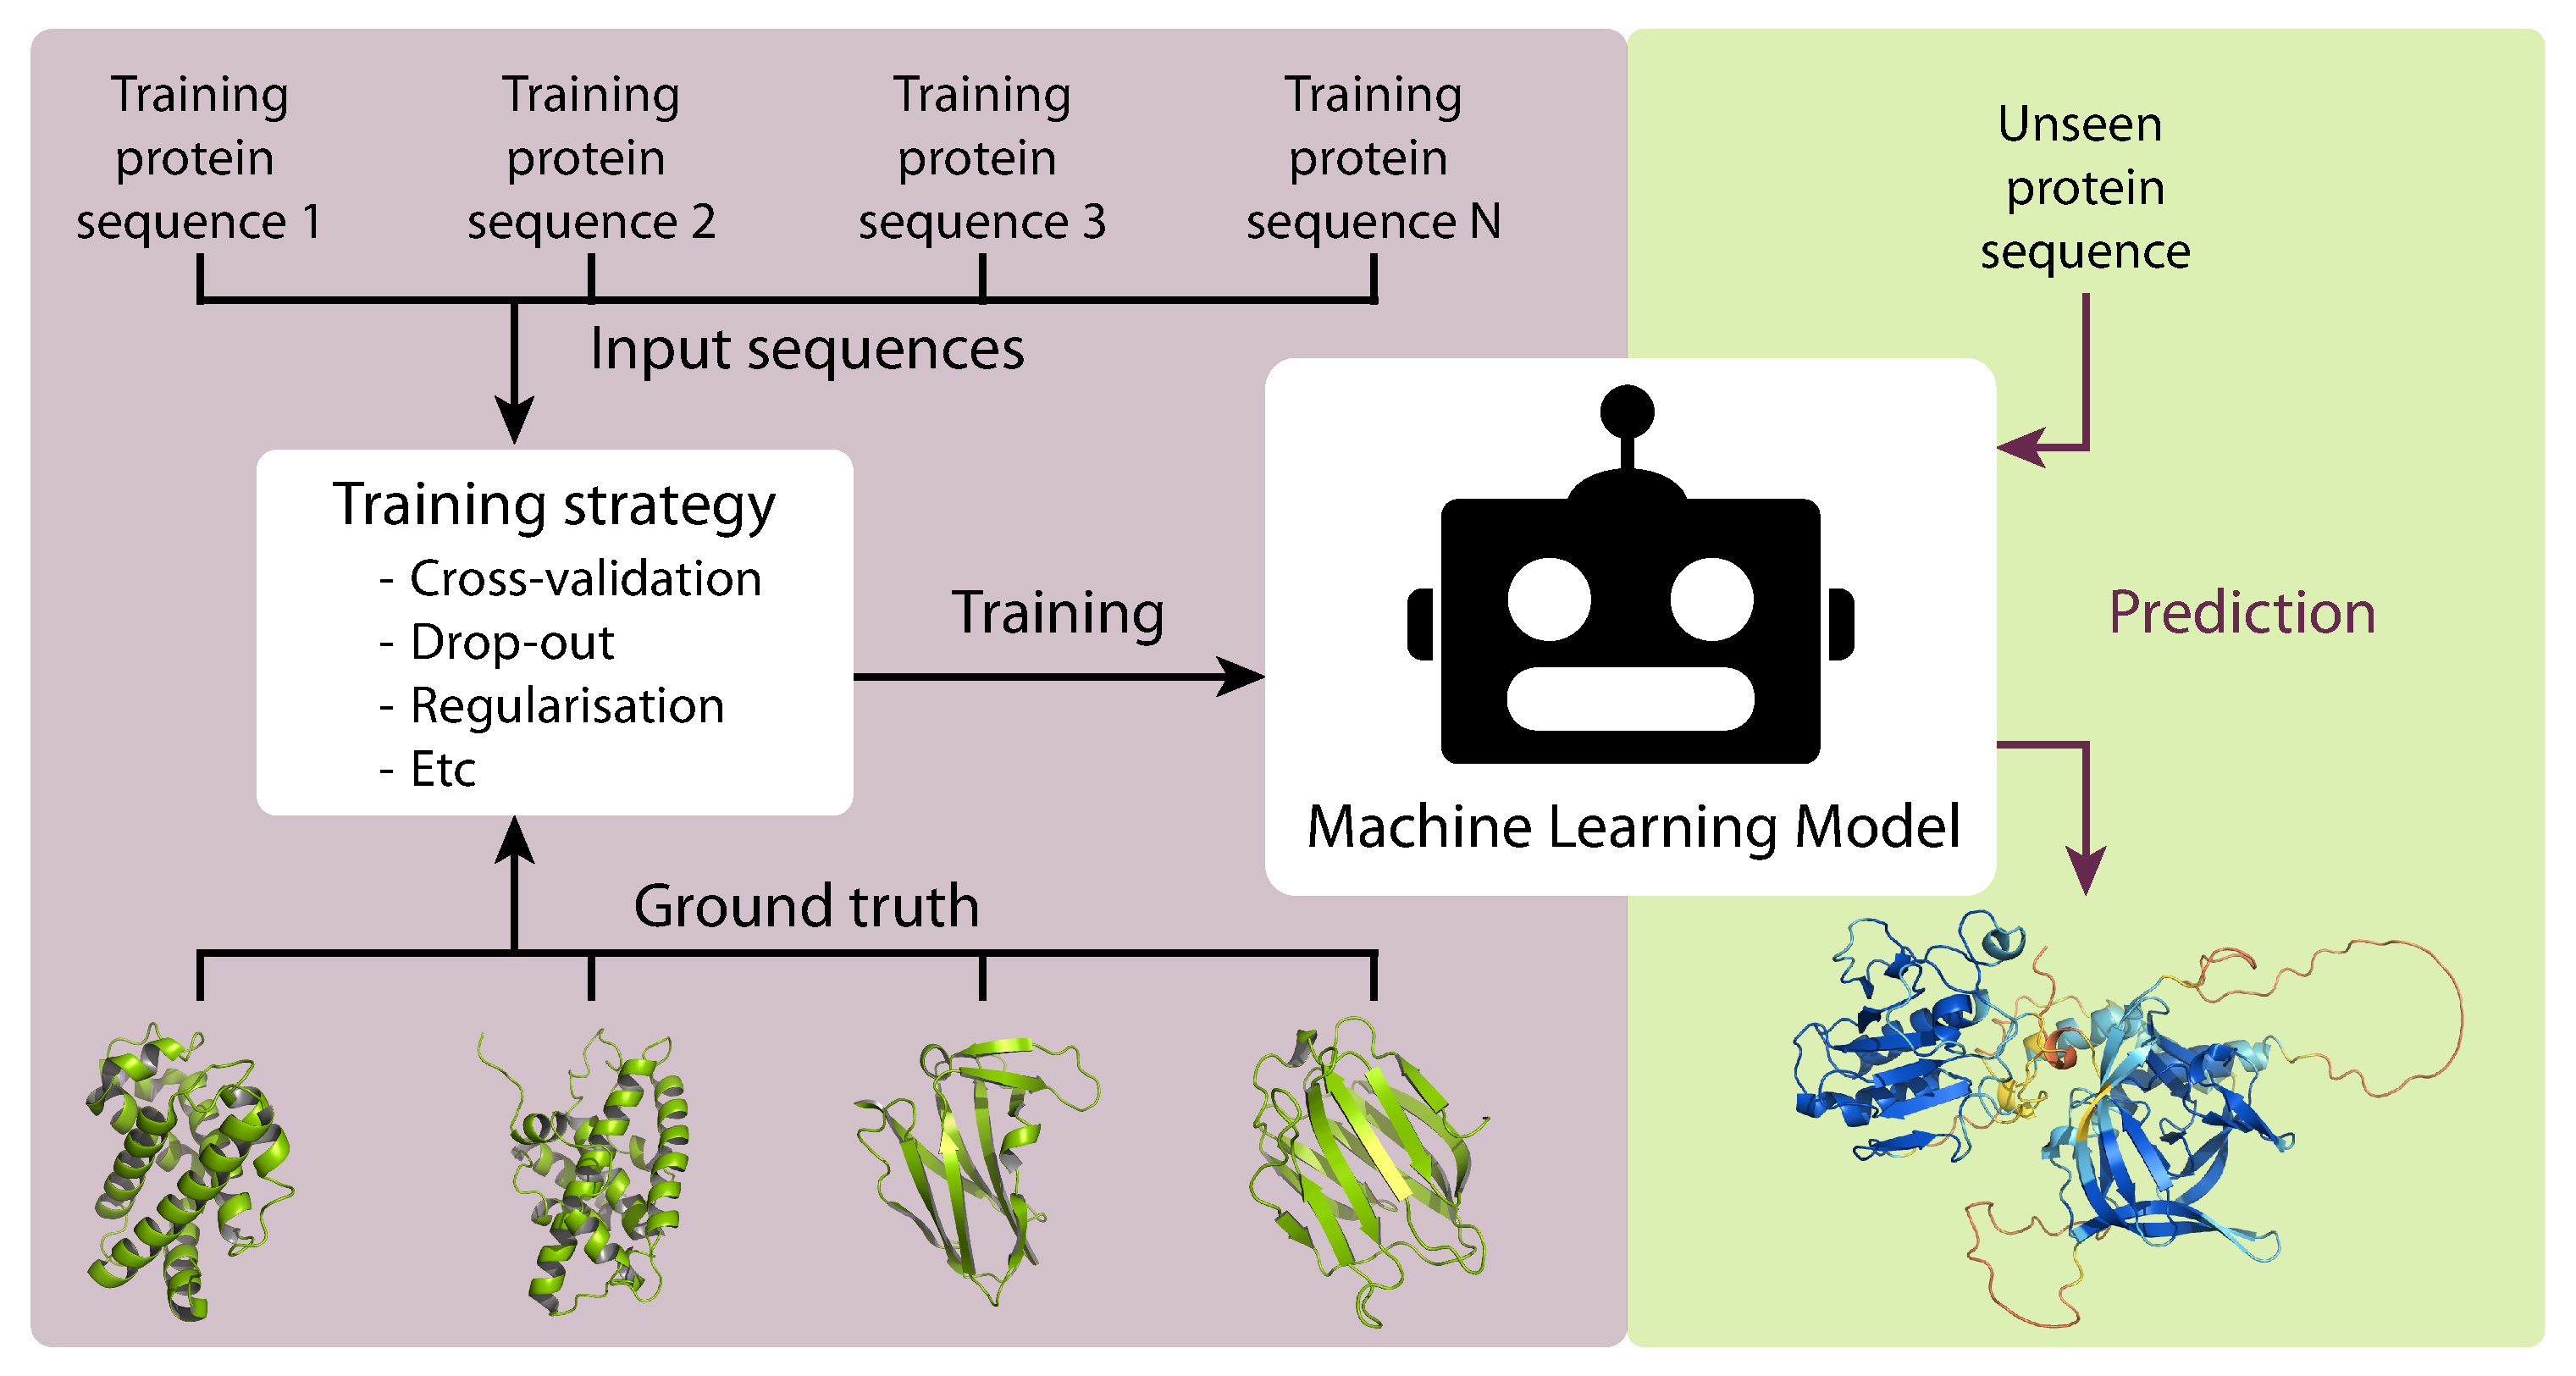
\includegraphics[width=0.95\linewidth]{figures/ml_basics.pdf}
    \caption{\textbf{Machine learning (\gls{machinelearning}) model basic training and prediction.} The general framework of a \glspl{supervisedlearning} \gls{machinelearning} model designed to predict \gls{proteinstructure} from its sequence uses as training data protein sequences and their corresponding \glspl{proteinstructure} as ground truths or expected outcomes. The training data is presented to the model according to the training strategy, which deploys methods to obtain a model able to correctly generalise (left). Strategies such as cross-validation prevent model ``overfitting'' (training data is learnt too well, capturing noise and details that do not generalise to new, unseen data, leading to poor performance on the latter). The trained model can then predict the structure of new, unseen protein sequences (right). \Glspl{proteinstructure} in the training diagram (left) with PDB IDs: 101M \cite{smith_robert_david_correlations_1999}, 1AD6 \cite{kim_structural_1997}, 1AKP \cite{constantine_sequential_1994}, and 1A3K \cite{seetharaman_x-ray_1998}. Predicted \gls{proteinstructure} (right) downloaded from \burl{https://alphafold.ebi.ac.uk/}, id Q15465.}
    \label{fig:chapter1:ml_basics}
\end{figure}


During the training process of \gls{supervisedlearning} models, the model adjusts its parameters, generally iteratively, to minimise the error between its predictions and the actual outcomes \cite{loog_chapter_2018}. The training process is assessed using metrics appropriate for the type of data. For discrete labels (\textit{e.g.} to classify whether a biological sample contains cancer), metrics such as \gls{accuracy}, \gls{precision}, \gls{recall}, and \Gls{f1score} \cite{naidu_review_2023} are used, while for continuous labels (\textit{e.g.} the prediction of a protein region's \gls{backbone} dynamics), metrics such as \Gls{meansquarederror}, \gls{rootmeansquarederror}, \gls{meanabsoluteerror}, and \gls{rsquared} \cite{botchkarev_performance_2019, chicco_coefficient_2021} provide insights into the model's performance.


\subsection{Sequence-Based Predictors}

A different approach to studying the dynamic nature of proteins using computational tools involves the use of \gls{machinelearning} models to estimate the values of diverse protein biophysical properties. Specifically, the use of sequence-based protein biophysics estimators, models that approximate the value of biophysical metrics from the \gls{aminoacid} sequence alone, is usually quick and inexpensive and allows for probing the expected features of a protein. A purely sequence-based estimator does not require the input of a \gls{proteinstructure}, thus permitting its use for screening and evaluating mutations for any position in the protein. The predictions obtained from these estimators can often be used as features for other models, as a kind of biophysical embedding or numerical description of \glspl{aminoacid} (Supplementary Table 4.2)
% (\supptableref{tab:tool_dependencies})
\cite{raimondi_exploring_2017, orlando_computational_2019, orlando_accurate_2020, orlando_prediction_2022}. In a set of aligned homologous sequences, they can be used to define the biophysically allowed space of a protein or protein family \cite{kagami_online_2021}. This can indicate key, near-immutable, protein regions as well as regions that are more robust to mutations that change biophysical behaviour. In both cases, this has clear implications for protein design and could be used either to introduce mutations which preserve or disrupt a biophysical behaviour, depending on the application. Our group, bio2Byte, has developed a suite of publicly available sequence-based predictors for protein biophysical properties (Chapter \ref{chapter:b2btools_deployment} \cite{gavalda-garcia_bio2byte_2024}).


\subsection{Interpretation of NMR Models with ShiftCrypt}

Another tool from our research group, though developed prior to this thesis, is ShifCrypt \cite{orlando_shiftcrypt_2020}. This tool uses an auto-encoder structure (or architecture, as it is a \gls{neuralnetworks}), a model that reduces the input vector size describing an input and attempts to reconstruct it from its minimum size \cite{lopez_pinaya_chapter_2020} (\textit{e.g.} a 100-dimensional input is converted into a 5-dimensional vector, from which the 100-dimensional vector is attempted to be reconstructed). ShiftCrypt is an auto-encoder that transforms the \glspl{chemicalshift} from an \gls{nmr} experiment into a single value per \gls{aminoacid}, which is its minimum vector size, to then attempt reconstruction of the input data (\figref{fig:chapter1:shiftcrypt}). This minimum size single value represents an \gls{aminoacid}'s biophysical space and indicates the range of secondary structures that a residue adopts in solution. It ranges from 0 to 1, representing pure Helix and Sheet \glspl{conformation} respectively. Near 0.5 values, the residue is \glspl{proteindisorder} and does not adopt any defined \gls{conformation}. Deviations from middle values indicate dynamic \glspl{conformation} with progressive tendencies towards Helix or Sheet. This method provides a simple interpretation of \gls{nmr} \glspl{chemicalshift} into a single, comprehensible value and is employed at multiple points during this thesis. 

\begin{figure}[tbh]
    \centering
    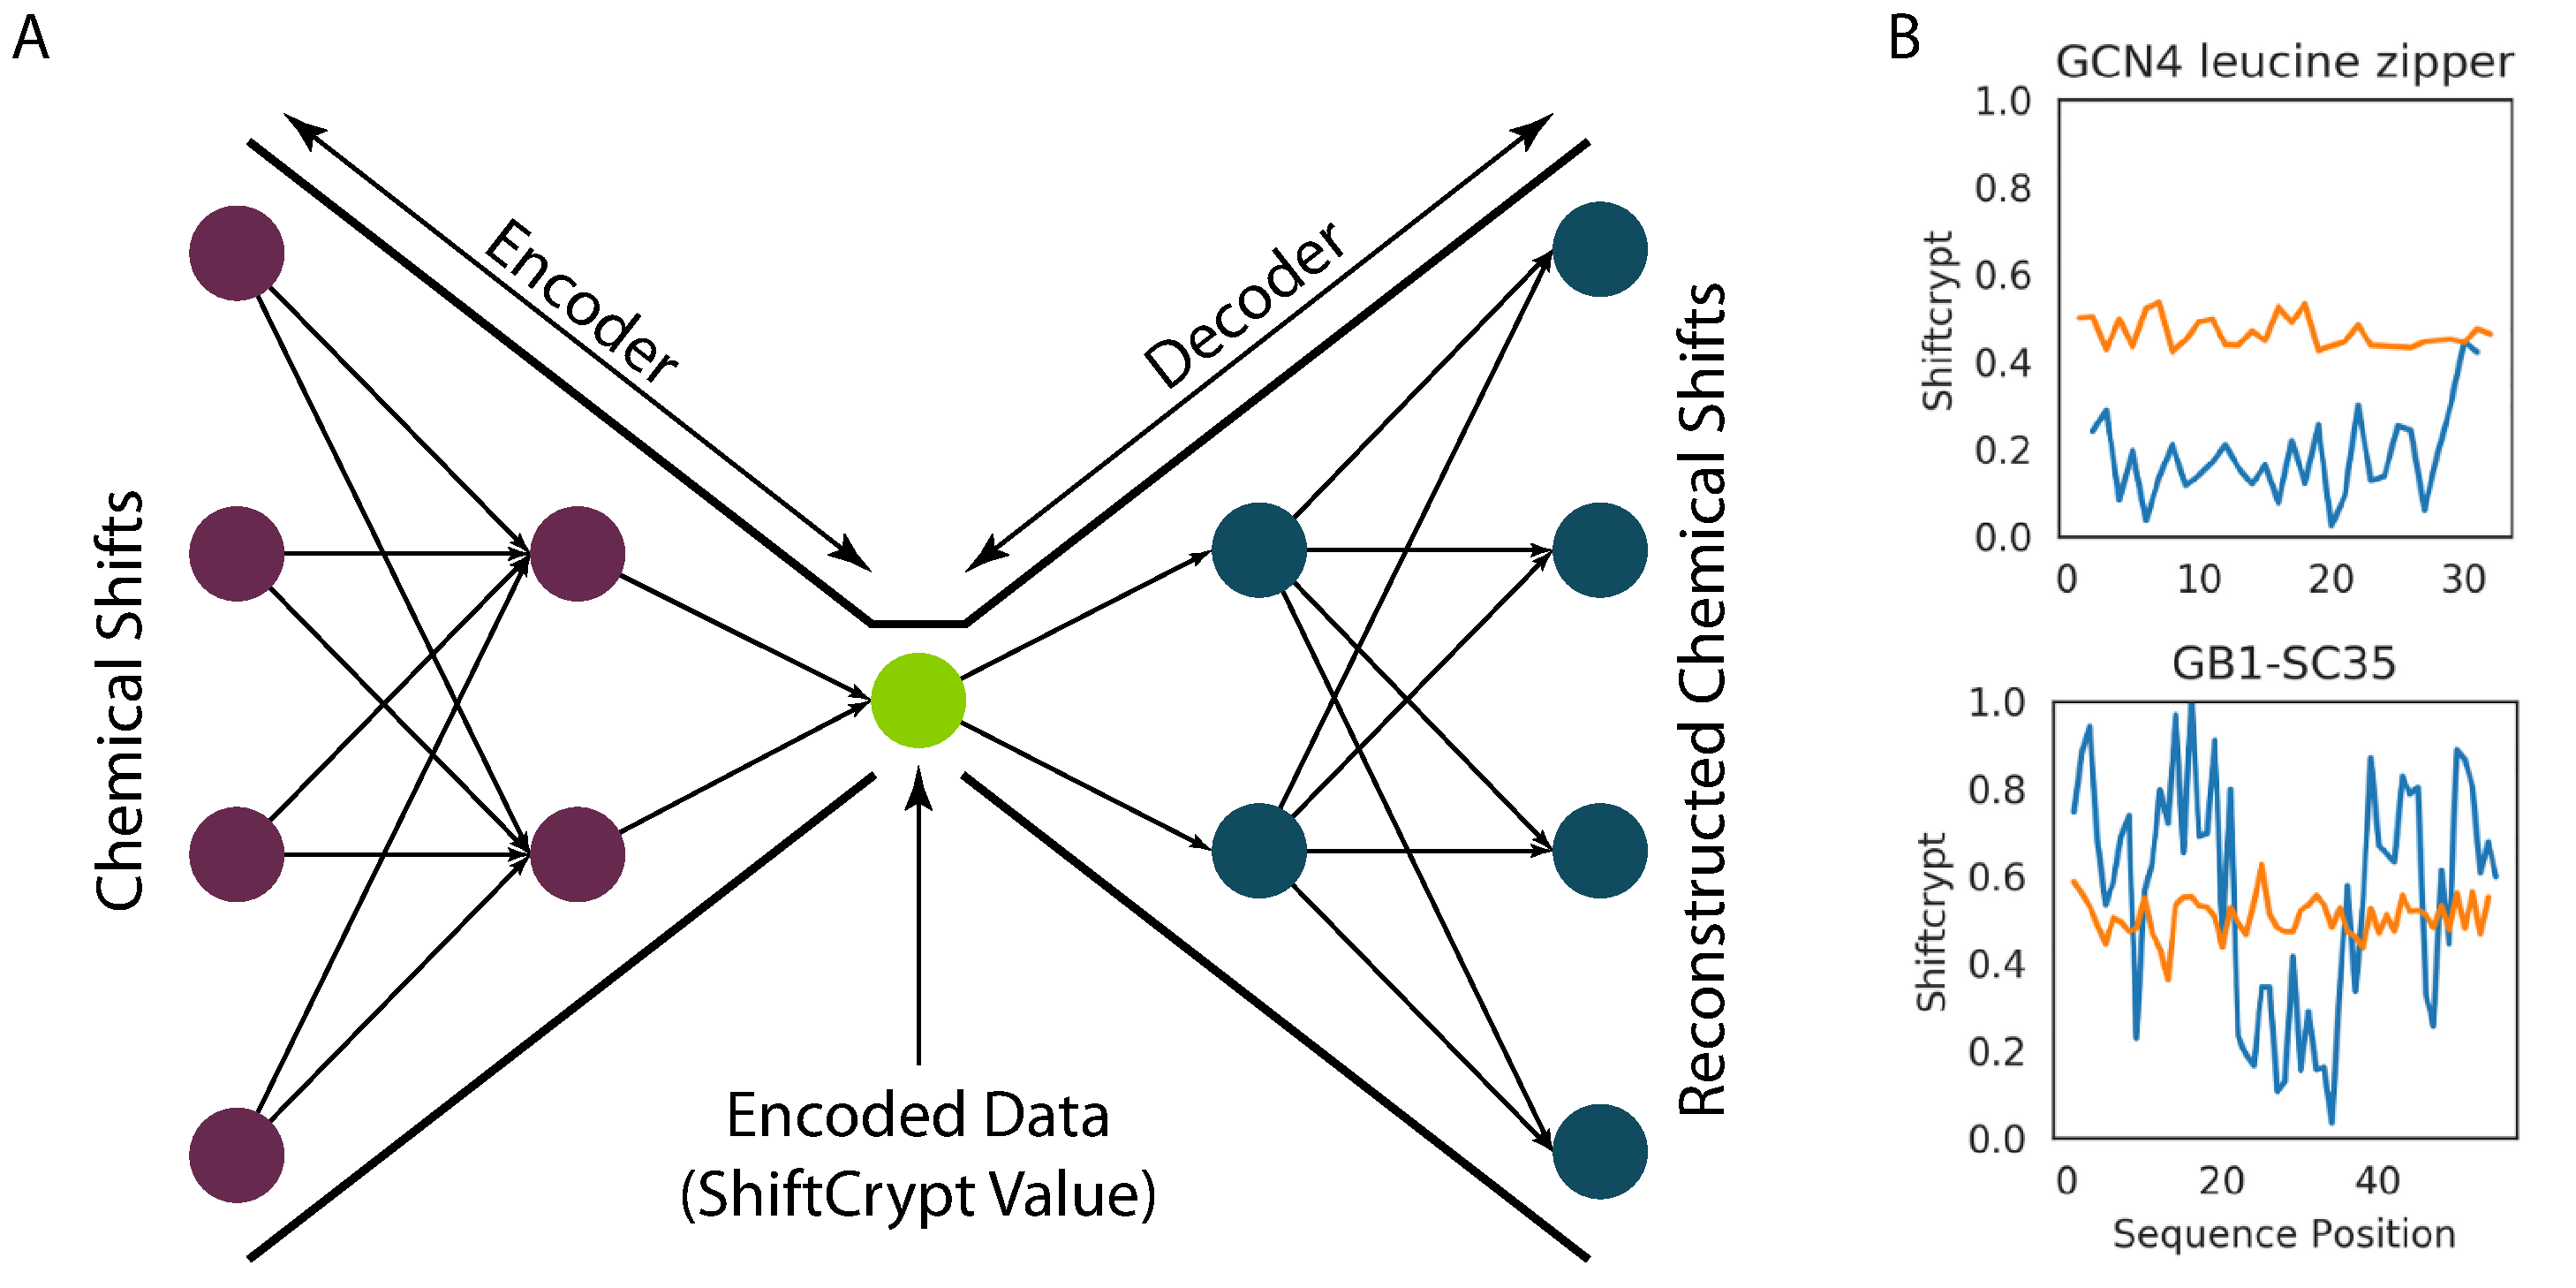
\includegraphics[width=1\linewidth]{figures/shiftcrypt.pdf}
    \caption{\textbf{ShiftCrypt auto-encoder architecture and \gls{proteindisorder} detection.} A) Schematic auto-encoder architecture of ShiftCrypt. The encoder section of the model transforms input \glspl{chemicalshift} into a single encoded value: the ShiftCrypt value. The decoder section of the model attempts to reconstruct the input \glspl{chemicalshift}. B) ShiftCrypt value for two proteins in presence (orange) and absence (blue) of urea. High concentrations of urea effectively denature a protein and causes to adopt a \glspl{proteindisorder} \gls{conformation}. For both proteins, the samples exposed to urea featured near 0.5 ShiftCrypt values, whereas the samples in absence of urea had more extreme values. This indicates that ShiftCrypt can detect absence and presence of fold, respectively. Subplot B extracted from \cite{orlando_shiftcrypt_2020}.}
    \label{fig:chapter1:shiftcrypt}
\end{figure}


\section{AlphaFold and its Relationship with Dynamics}

Over decades, the combined efforts of the structural biology community painstakingly elucidated individual \glspl{proteinstructure}, has resulted in the deposition of over 220,000 \glspl{proteinstructure} in the Protein Data Bank \cite{noauthor_pdb_nodate}. Due to the difficulties in obtaining such data, \gls{proteinstructure} prediction became a prominent field of bioinformatics, with bi-annual editions of the Critical Assessment of Structure Prediction (CASP) judging the state of the field \cite{moult_large-scale_1995}. During CASP, a set of protein sequences with experimentally elucidated but unpublished structures is given to all participants. The predictions from all participants are scored on the prediction of 
protein structures belonging to different categories, according to the protein's difficulty and/or characteristics. This allows to determine which predictive methods work better for each predictive task and quantify their prediction's quality.

Traditionally, protein structural prediction relied on diverse knowledge-based or empirical methods based on statistical and computational techniques, often used in combination. One of these techniques is fragment assembly, where the protein's \gls{aminoacid} sequence is divided into short fragments, typically 3-9 residues long. These fragments are then matched with similar sequences in a database of known \glspl{proteinstructure} to find possible \glspl{conformation} \cite{rohl_protein_2004}. The chosen fragments are assembled into a full \gls{proteinstructure} using an optimisation algorithm to minimise an energy function, which ensures the most likely stable \gls{conformation}. One of these algorithms is the optimisation by \glspl{montecarlosimulations}, a technique that uses random sampling to explore possible configurations and energies of the protein \cite{rohl_protein_2004}. One of the simplest manners to apply \glspl{montecarlosimulations} for \gls{proteinstructure} determination is to randomly change the location of an \gls{aminoacid} and evaluate the free energy of each derived structure. In replica exchange \glspl{montecarlosimulations} \cite{xu_ab_2012}, a series of \glspl{montecarlosimulations} are performed in parallel at different temperatures. The samples are exchanged among different temperatures, which allows for searching an energy \gls{globalminima} at low temperatures and overcome \glspl{localminima} (\figref{fig:chapter1:landscape}) at high temperatures, thereby finding a lower energy minimum solution for the \gls{proteinstructure} \cite{xu_ab_2012}. These simulations require an initial structure to sample, which can be a random coil in its most naïve form or an expected nearer \gls{conformation}, like the \gls{conformation} of a homologous protein or a predicted \gls{conformation} obtained from the previously explained fragment assembly \cite{yang_i-tasser_2015}.


Then, DeepMind's AlphaFold brought a \gls{machinelearning} approach to the assessment, profiting from Protein Data Bank and UniProt databases to train their model \cite{senior_improved_2020}. Two years later, it achieved near-experimental resolution \cite{jumper_highly_2021} for monomeric structures. The large size of the databases employed to create its training set permitted the use of \glspl{deepneuralnetworks}(DNN), which feature multiple high-dimensional layers, generally with complex architectures and activation functions.


AlphaFold2 used both protein sequence and structure data for its training. It used all then available sequences on UniProt, which were filtered for redundancy and aligned in Multiple Sequence Alignments (\gls{msa}). It also generates a pair representation, a matrix with vectors describing the relationship of each \gls{aminoacid} in the input protein with every other \gls{aminoacid}. Both of these were employed to train a series of \gls{attention}-based modules named ``Evoformers'' \cite{vaswani_attention_2023,jumper_highly_2021}, essential for understanding secondary structure elements like \glspl{alphahelix} and \glspl{betasheet}, or structures spanning distant regions, due to the different focus ranges employed (\textit{i.e.} it learns both short- and long-range interactions). In the \gls{msa}, \gls{attention}, an 
advanced feature extraction \gls{machinelearning} method, is applied across the totality of a single sequence to capture patterns within a protein itself, and across a single position in all proteins in the \gls{msa} to capture evolutionary relationships in all aligned proteins. In the pair representation, 2-dimensional \gls{attention} is employed to learn local and global geometric interactions among all \glspl{aminoacid}. This is followed by structure modules, which estimate the protein's 3-dimensional structure from the output of the Evoformer, which is compared with the reference PDB structure during the training process. This process is refined by recycling the data and feeding it back into the network three times (by default), so structural (from PDB) and evolutionary (from \gls{msa}) information is interconnected \cite{jumper_highly_2021} (\figref{fig:chapter1:af2_structure}).

\begin{figure}[H]
    \centering
    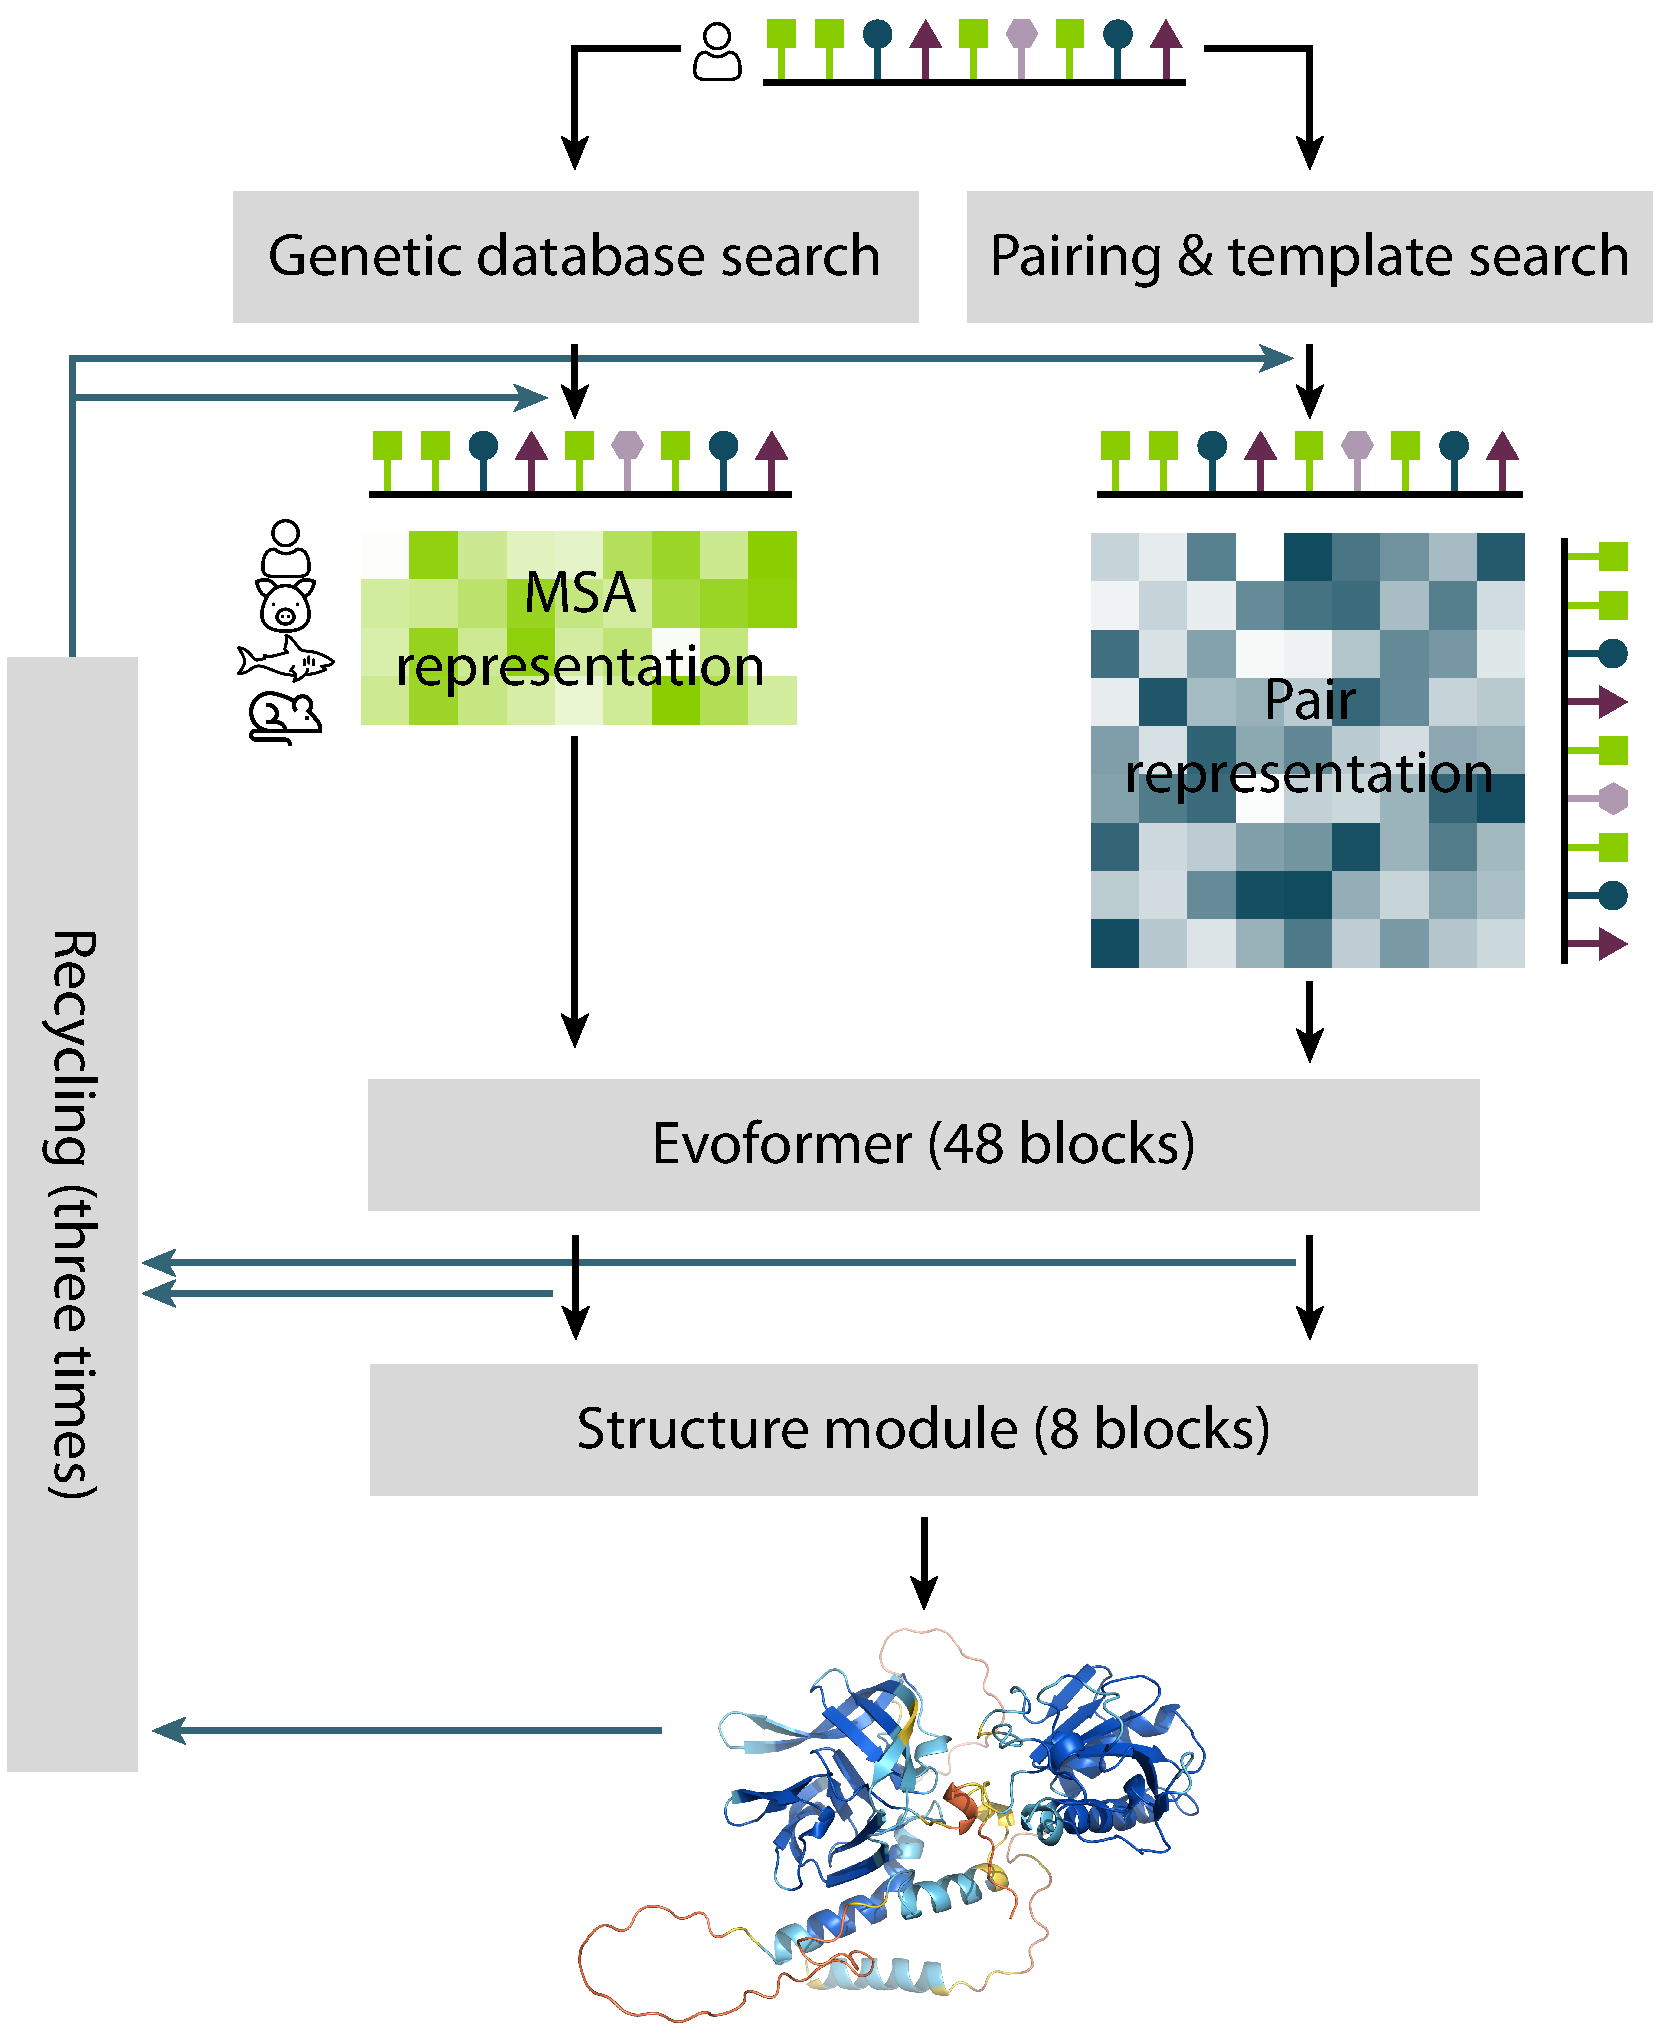
\includegraphics[width=0.75\linewidth]{figures/af2_architecture_simple.pdf}
    \caption{\textbf{AlphaFold2's \gls{neuralnetworks} simplified architecture and training process.} AlphaFold2 takes a protein sequence as input, a human sequence in this example. This sequence is queried against a sequence database to find homologous sequences and align them and create an \gls{msa} representation (left, green matrix). It is also used to create a pair representation (right, blue matrix) and to query a structural database to find suitable templates to facilitate structural modelling (not shown in figure). Both representations are passed through 48 \gls{attention}-based Evoformer blocks, followed by 8 structure module blocks. This produces a predicted structure. The outputs from the Evoformer and structure module blocks are recycled and fed into the \gls{msa} and pair representation 3 times, to refine the results. Figure adapted and simplified from \cite{jumper_highly_2021}. \gls{proteinstructure} downloaded from \burl{https://alphafold.ebi.ac.uk/}, id Q15465. Human and animal icons licensed by \burl{https://www.flaticon.com}.}
    \label{fig:chapter1:af2_structure}
\end{figure}

The predicted structures are accompanied by two quality metrics: the predicted local distance difference test (\gls{plddt}) and the predicted aligned error (\gls{pae}). \gls{plddt} is a local metric of predictive confidence expressed as a single value per \gls{aminoacid}, whereas \gls{pae} is a 2-dimensional matrix that indicates the certainty of two residues to be predicted at a correct distance from each other \cite{jumper_highly_2021}. \gls{plddt} was studied as part of this thesis, in relation to different metrics of protein \gls{dynamics}, in chapter \ref{chapter:plddt}, for which we concluded that high and low \gls{plddt} values tend to correlate with protein \gls{flexibility} and \gls{dynamics}, but their gradations are not accurately predicted by \gls{plddt} values. 

Importantly, only the PDB structures obtained from \gls{xraycrystallography} crystallography and \gls{cryoem} were used for training, and any \glspl{ligand} were removed pre-training. This decision results in two important considerations: firstly, the exclusion of \gls{nmr}-derived structures biases the predictions towards more rigid \glspl{conformation} that a protein would obtain in \gls{physiologicalconditions}. Secondly, the removal of \glspl{ligand} results in predicted structures with empty chemical pockets, whose rigidity can be overestimated to the extent that derivative models are able to place the missing \gls{ligand} \cite{hekkelman_alphafill_2023}.


The third iteration of AlphaFold has recently been released \cite{abramson_accurate_2024}, which now allows for the inclusion of ions, small molecules, nucleic acids, and modified \glspl{aminoacid} in the predictions. It also shows improvement in protein complex prediction compared with its previous version. We show in chapter \ref{chapter:plddt} that the relation of AlphaFold3 \gls{plddt} of the $\alpha\text{-carbon}$ with protein \gls{dynamics} and \gls{flexibility} is comparable to that of AlphaFold2 for a reduced set of proteins. We were unable to perform the full large-scale analysis for AlphaFold3, as DeepMind had unfortunately not released the model's source code \cite{noauthor_alphafold3_2024} until days before the submission of this thesis \cite{callaway_ai_2024} and the stringent submission caps to their servers prevented such analysis. This contrasts with the open science requirements that journals have enforced in recent years and has left the community disappointed with Nature's non-enforcement for this specific case \cite{lin_alphafold_2024, wankowicz_alphafold3_2024}.

\section{Open Science and Tool Deployment}

Science has become increasingly open, particularly in the last decade, in order to fight the still ongoing crisis of reproducibility and to ensure that data, tools and methods developed during a project can be used beyond publication day. Funding institutions like the European Commission now require the open publication of derived data, publications, and any other research outcomes. Following this trend, most scientific journals now also require the public deposition of a project’s code and data before even considering publication, with the recent exception of Nature, which did not enforce such requirements by the publication date of DeepMind’s AlphaFold3  \cite{noauthor_alphafold3_2024}.

As a result of science’s move towards greater openness, the FAIR principles (\Gls{findability}, \Gls{accessibility}, \Gls{interoperability}, and \Gls{reusability}) were postulated to allow data have a second life beyond publication \cite{jacobsen_fair_2020}. Not every data set can fully comply with all principles (\textit{e.g.} there is no standard database to collect the specific kind of generated data), but the aim should be to achieve the highest possible compliance. To facilitate this, tools like ELIXIR's Data Stewardship Wizard \cite{pergl_data_2019, devignes_experiences_2023} have been published, which encourage researchers to plan and evaluate their research data management plans to maximise their FAIR score.

Nowadays, these principles are applied not only to data but have also expanded into \glspl{machinelearning} models, manuscripts, and scientific software development. Chapter \ref{chapter:b2btools_deployment} illustrates the efforts made in this thesis to improve the FAIR status of our group's suite of protein biophysical predictors, bio2Byte Tools \cite{gavalda-garcia_bio2byte_2024}. 

% \section{Before you read the remainder of this thesis}
% The work in this thesis is the culmination of 5 years of research at the bio2Byte group, under Wim Vranken's supervision. Following this introduction, I discuss the scientific and societal context of this work, together with my personal contributions to each project in this thesis. This is followed by a collection of articles produced during this period, which represent the main work of the thesis. The vision of the bio2Byte group has clearly influenced me as a researcher, and by extension the contents of this thesis, and one key, unifying concept must be kept in mind for its full understanding: proteins are dynamic entities with no single, static conformation.

% Enjoy the read.
